
\subsection{Plotted Limits}
%%%%%%%%%%%%%%%%%%%%%%%%%%%%%%

\subsubsection{Zero-Jet Cut-Based}
\begin{figure}[!htbp]
\centering
\subfigure[]{
\centering
\label{subfig:lp_0j_sf_cut}
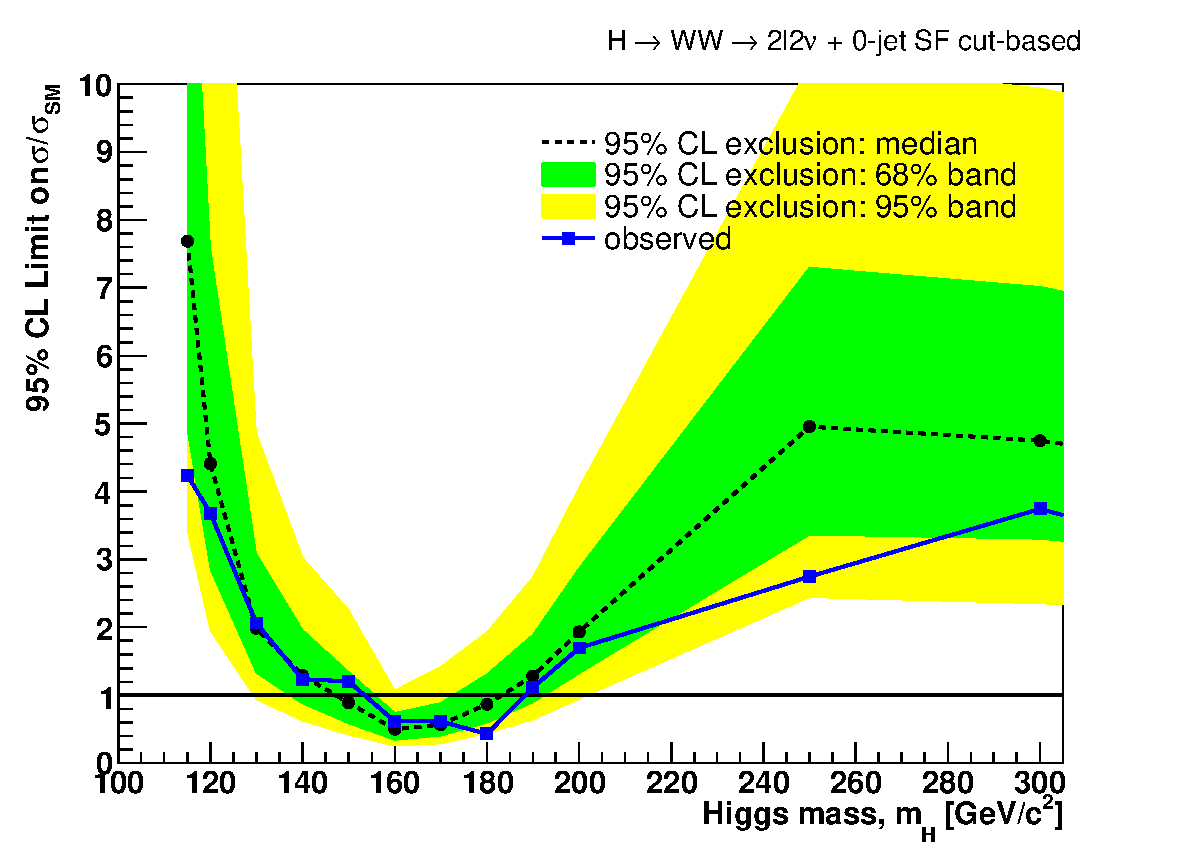
\includegraphics[width=0.48\textwidth]{lp_figures/limits_0j_sf_cut.pdf}}
\subfigure[]{
\centering
\label{subfig:lp_0j_of_cut}
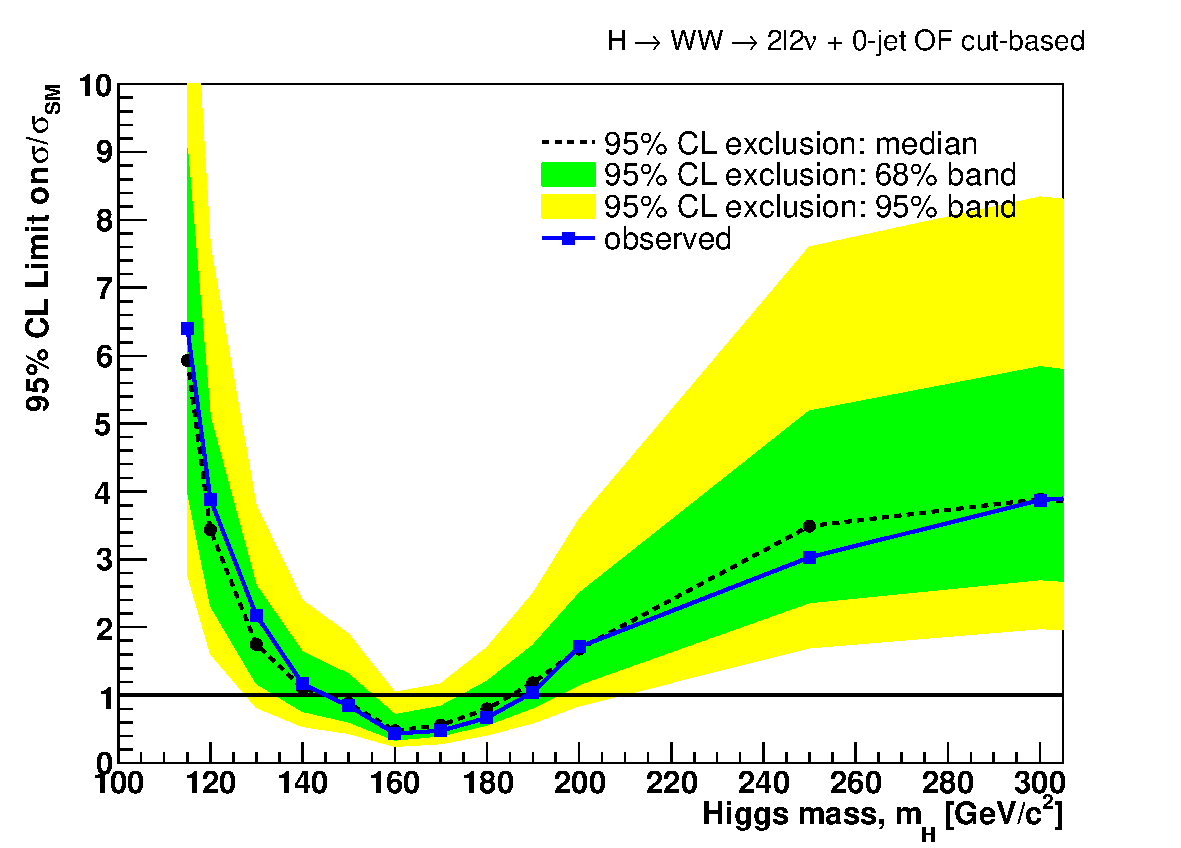
\includegraphics[width=0.48\textwidth]{lp_figures/limits_0j_of_cut.pdf}}
\subfigure[]{
\centering
\label{subfig:eps_0j_sf_cut}
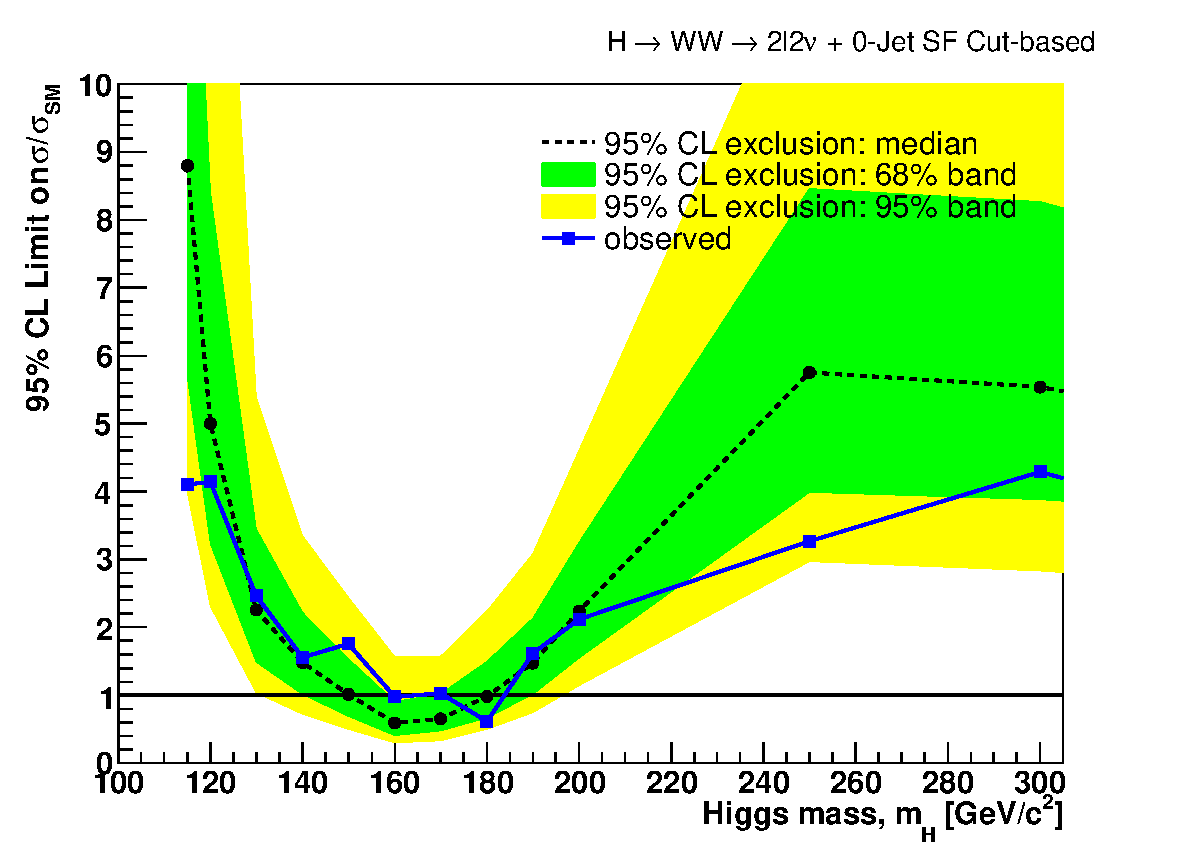
\includegraphics[width=0.48\textwidth]{lp_figures/limits_0j_sf_cut_ana_v6_1500pb_LP_EPS.pdf}}
\subfigure[]{
\centering
\label{subfig:eps_0j_of_cut}
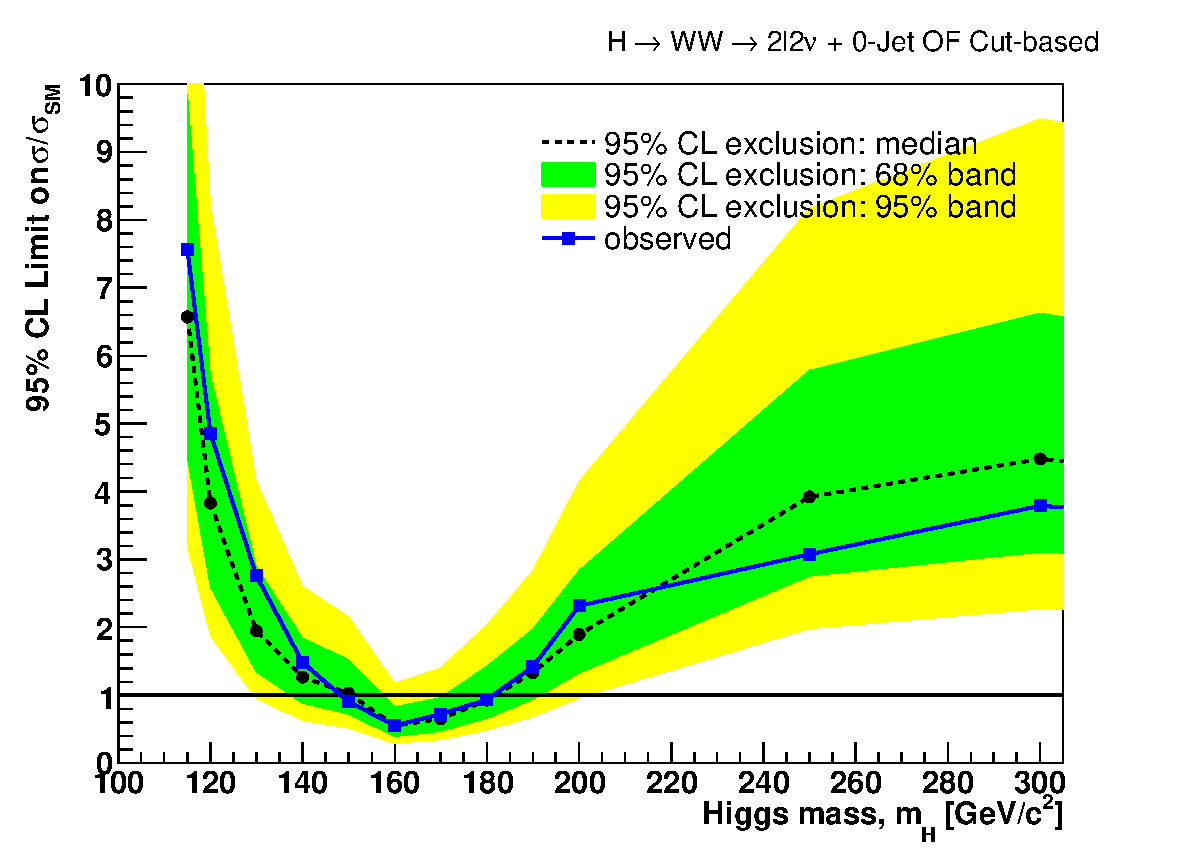
\includegraphics[width=0.48\textwidth]{lp_figures/limits_0j_of_cut_ana_v6_1500pb_LP_EPS.pdf}}
\subfigure[]{
\centering
\label{subfig:post_0j_sf_cut}
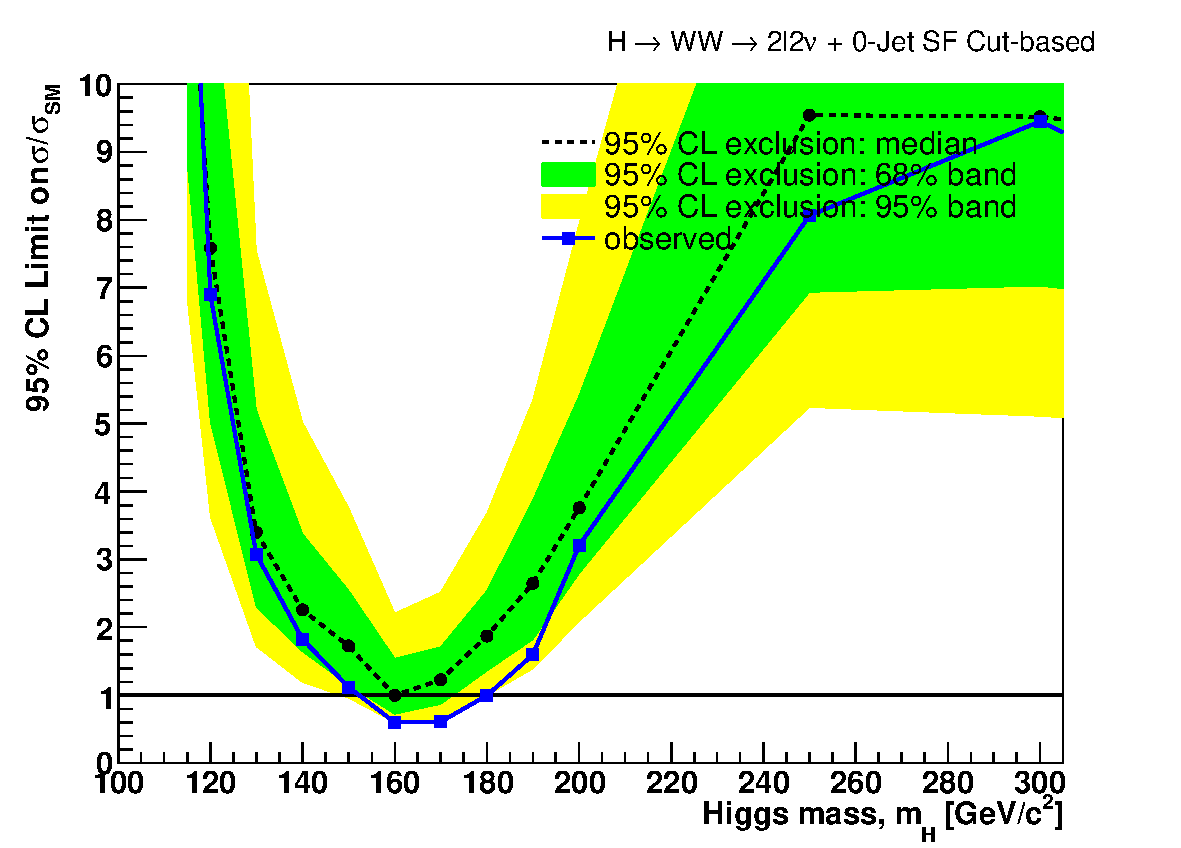
\includegraphics[width=0.48\textwidth]{lp_figures/limits_0j_sf_cut_ana_v6_1500pb_LP_POSTEPS.pdf}}
\subfigure[]{
\centering
\label{subfig:post_0j_of_cut}
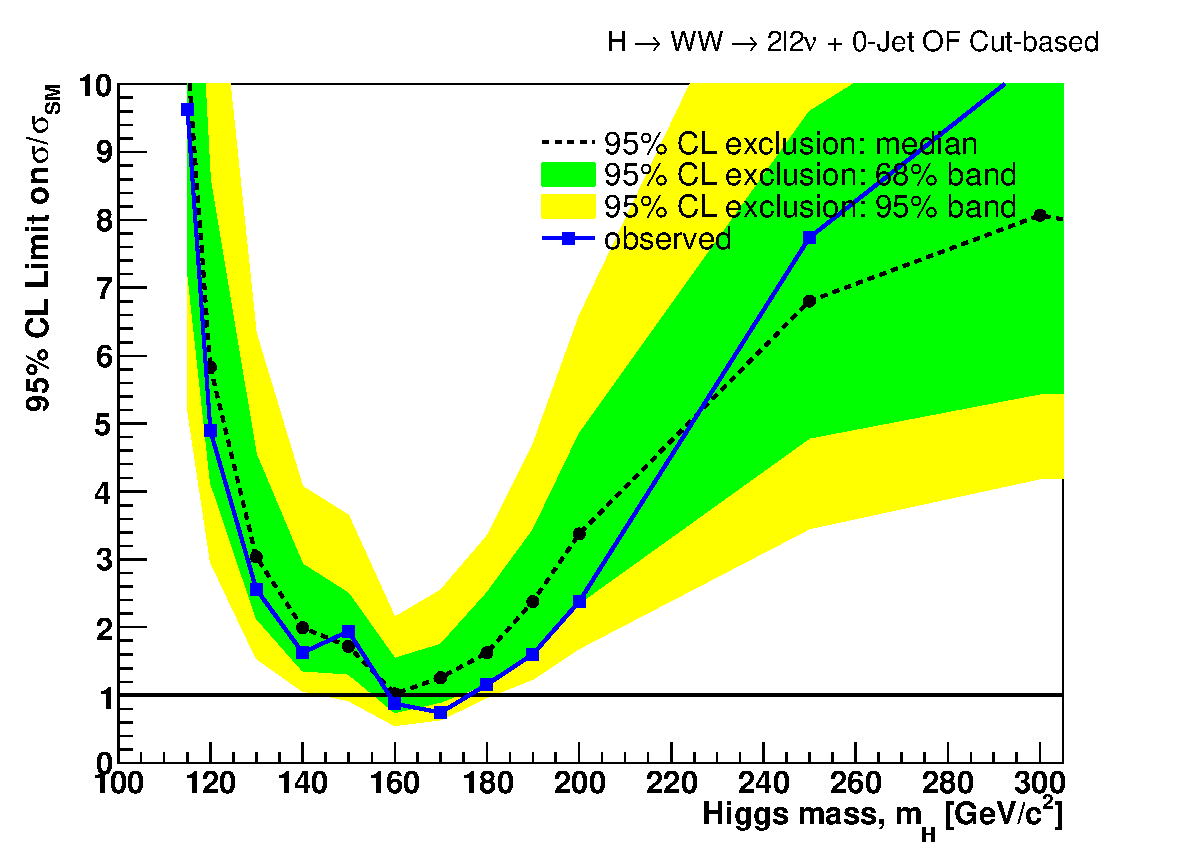
\includegraphics[width=0.48\textwidth]{lp_figures/limits_0j_of_cut_ana_v6_1500pb_LP_POSTEPS.pdf}}
\caption{Cut-based analysis upper limits at 95\% C.L. using LP, EPS and post-EPS datasets for 0-jet events.
\subref{subfig:lp_0j_sf_cut}: LP same-flavor; \subref{subfig:lp_0j_of_cut}: LP opposite-flavor;
\subref{subfig:eps_0j_sf_cut}: EPS same-flavor; \subref{subfig:eps_0j_of_cut}: EPS opposite-flavor;
\subref{subfig:post_0j_sf_cut}: post-EPS same-flavor; \subref{subfig:post_0j_of_cut}: post-EPS opposite-flavor;
}
\label{fig:limits_0j_cut}
\end{figure}

\subsubsection{Zero-Jet MVA-Based}
\begin{figure}[!htbp]
\centering
\subfigure[]{
\centering
\label{subfig:lp_0j_sf_shape}
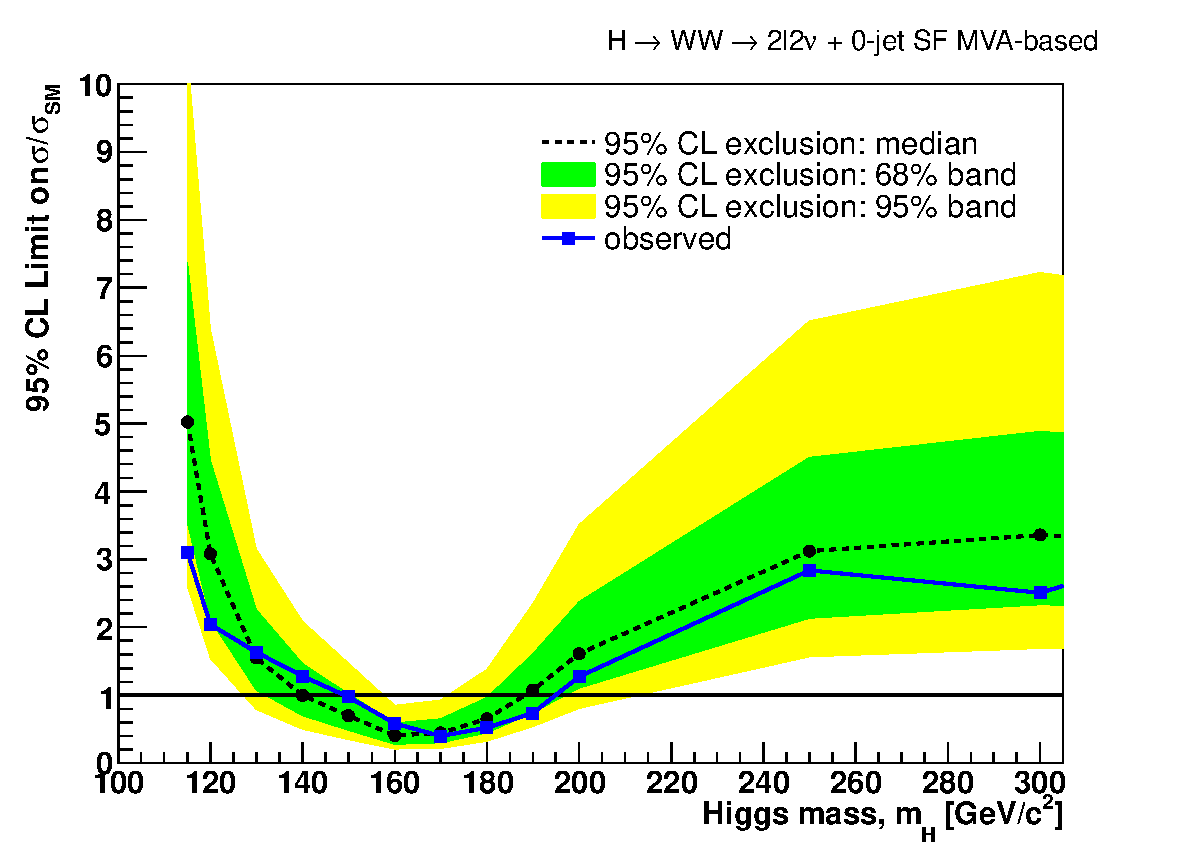
\includegraphics[width=0.48\textwidth]{lp_figures/limits_0j_sf_shape.pdf}}
\subfigure[]{
\centering
\label{subfig:lp_0j_of_shape}
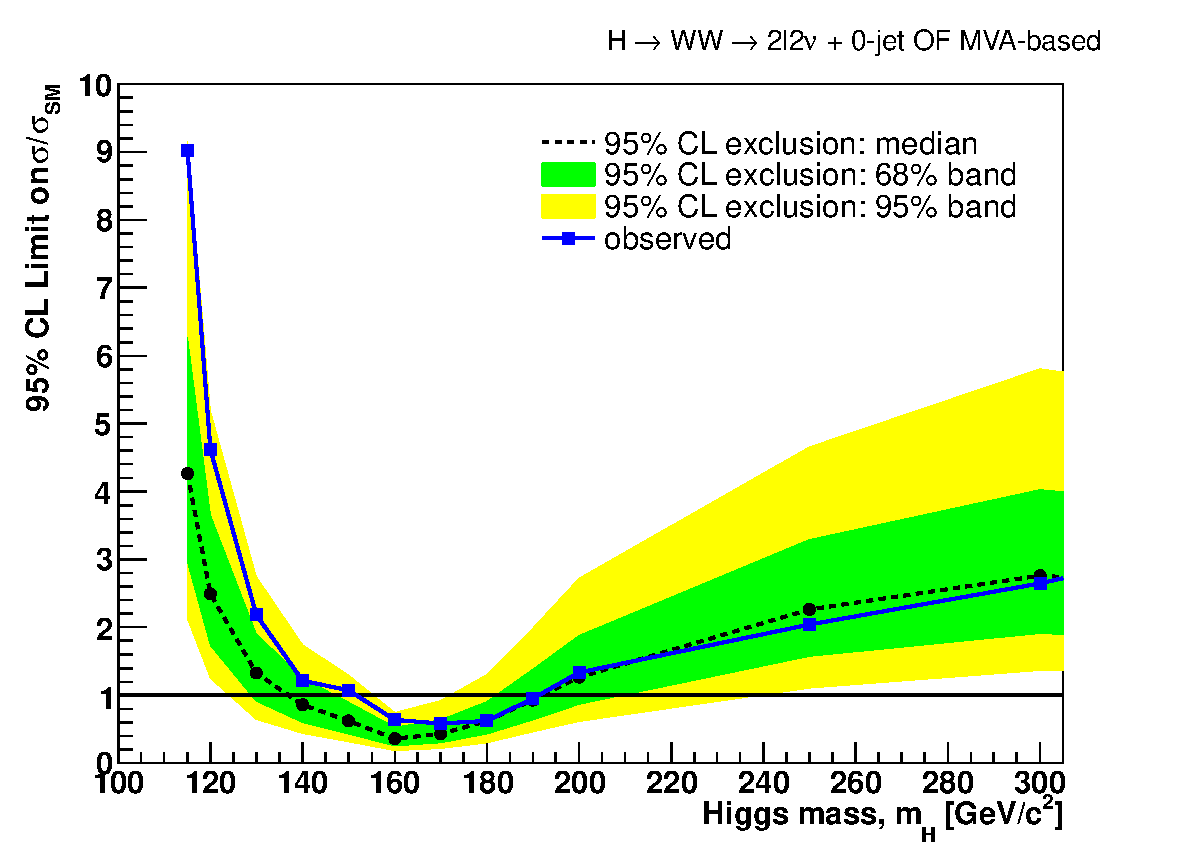
\includegraphics[width=0.48\textwidth]{lp_figures/limits_0j_of_shape.pdf}}
\subfigure[]{
\centering
\label{subfig:eps_0j_sf_shape}
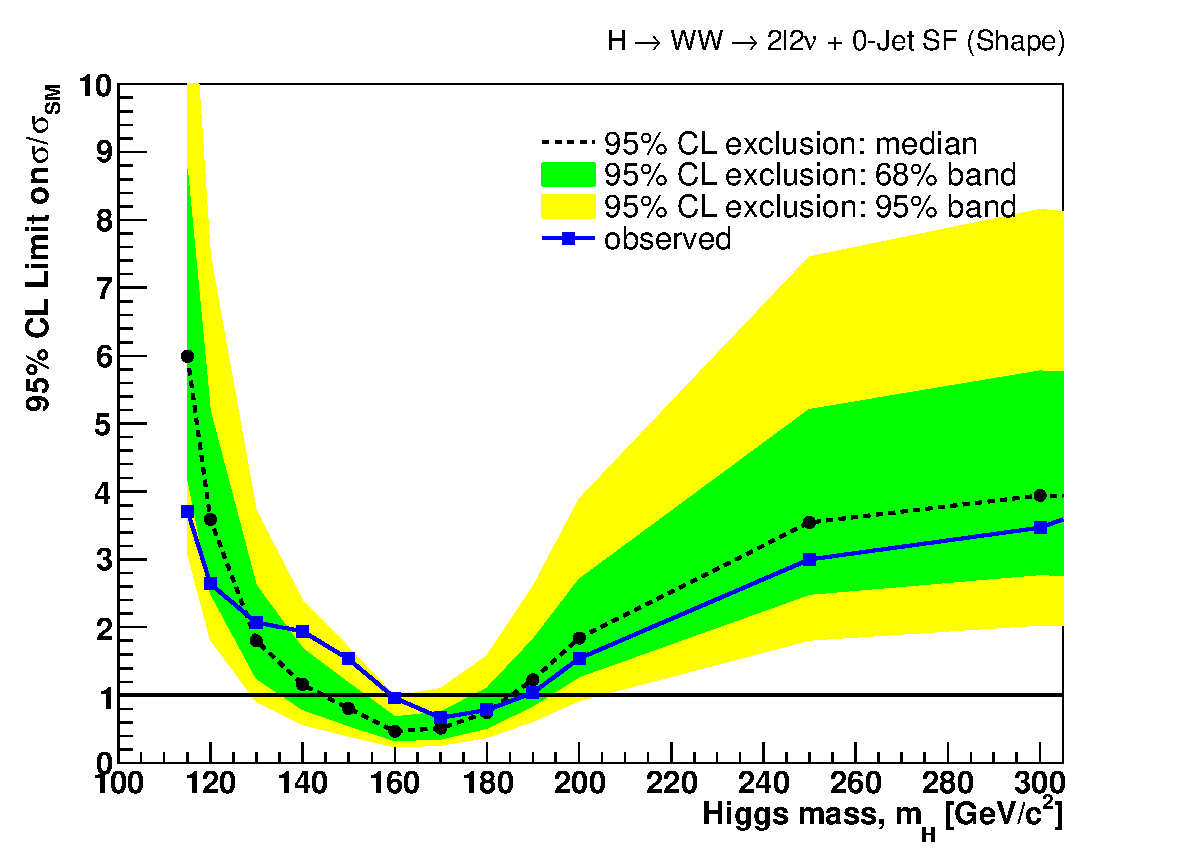
\includegraphics[width=0.48\textwidth]{lp_figures/limits_0j_sf_shape_ana_v6_1500pb_LP_EPS.pdf}}
\subfigure[]{
\centering
\label{subfig:eps_0j_of_shape}
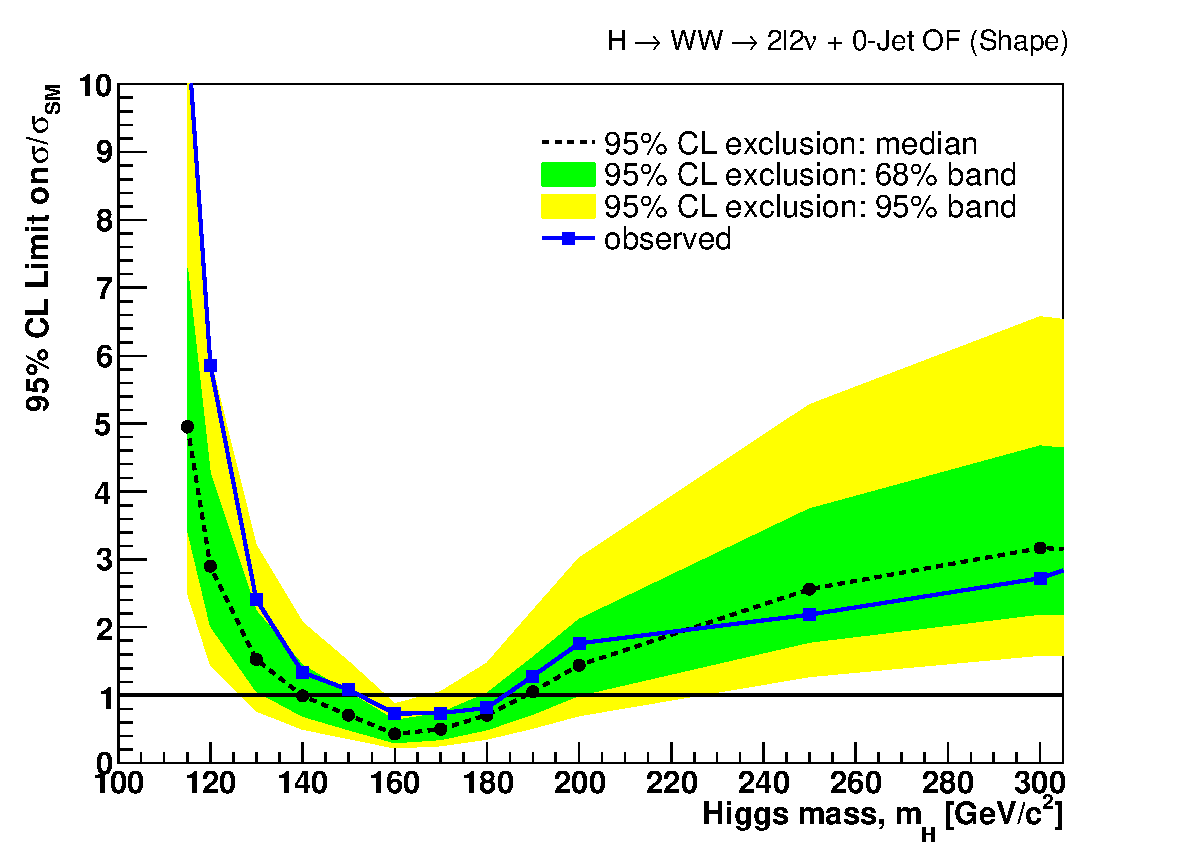
\includegraphics[width=0.48\textwidth]{lp_figures/limits_0j_of_shape_ana_v6_1500pb_LP_EPS.pdf}}
\subfigure[]{
\centering
\label{subfig:post_0j_sf_shape}
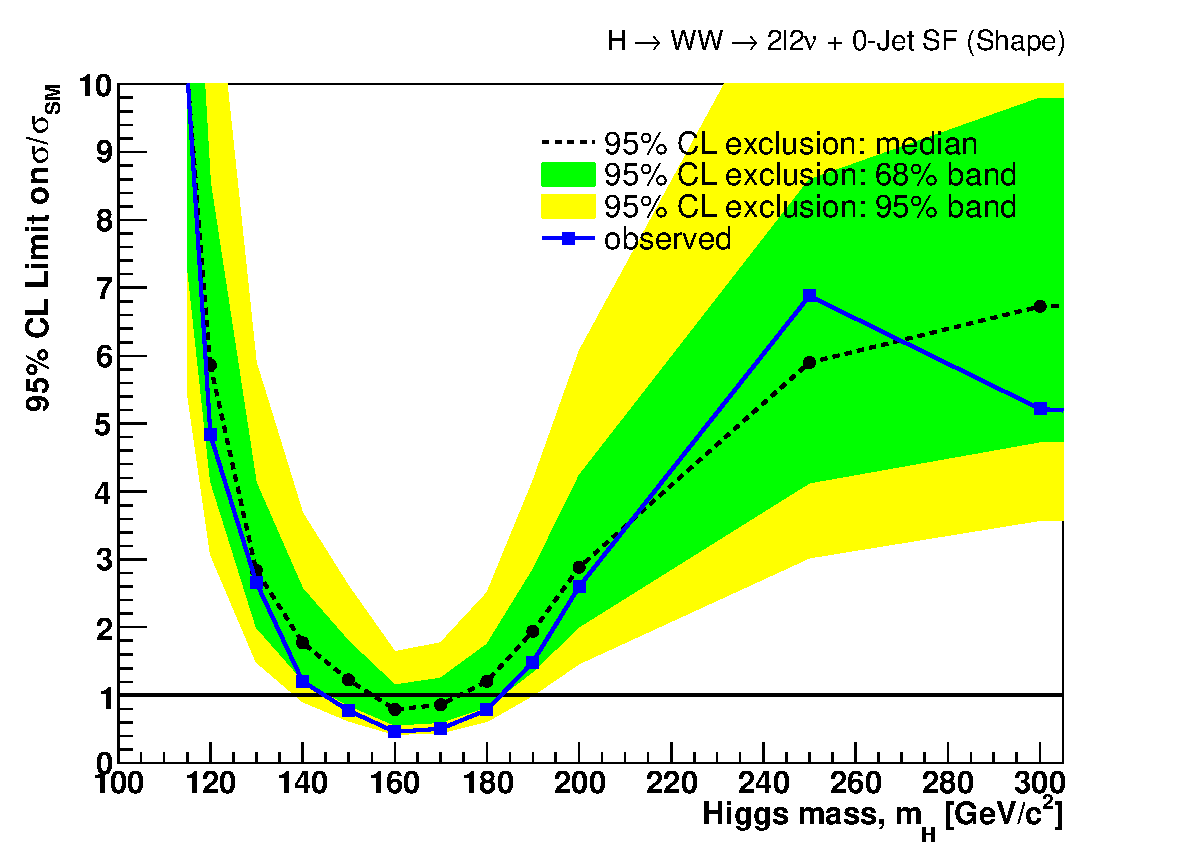
\includegraphics[width=0.48\textwidth]{lp_figures/limits_0j_sf_shape_ana_v6_1500pb_LP_POSTEPS.pdf}}
\subfigure[]{
\centering
\label{subfig:post_0j_of_shape}
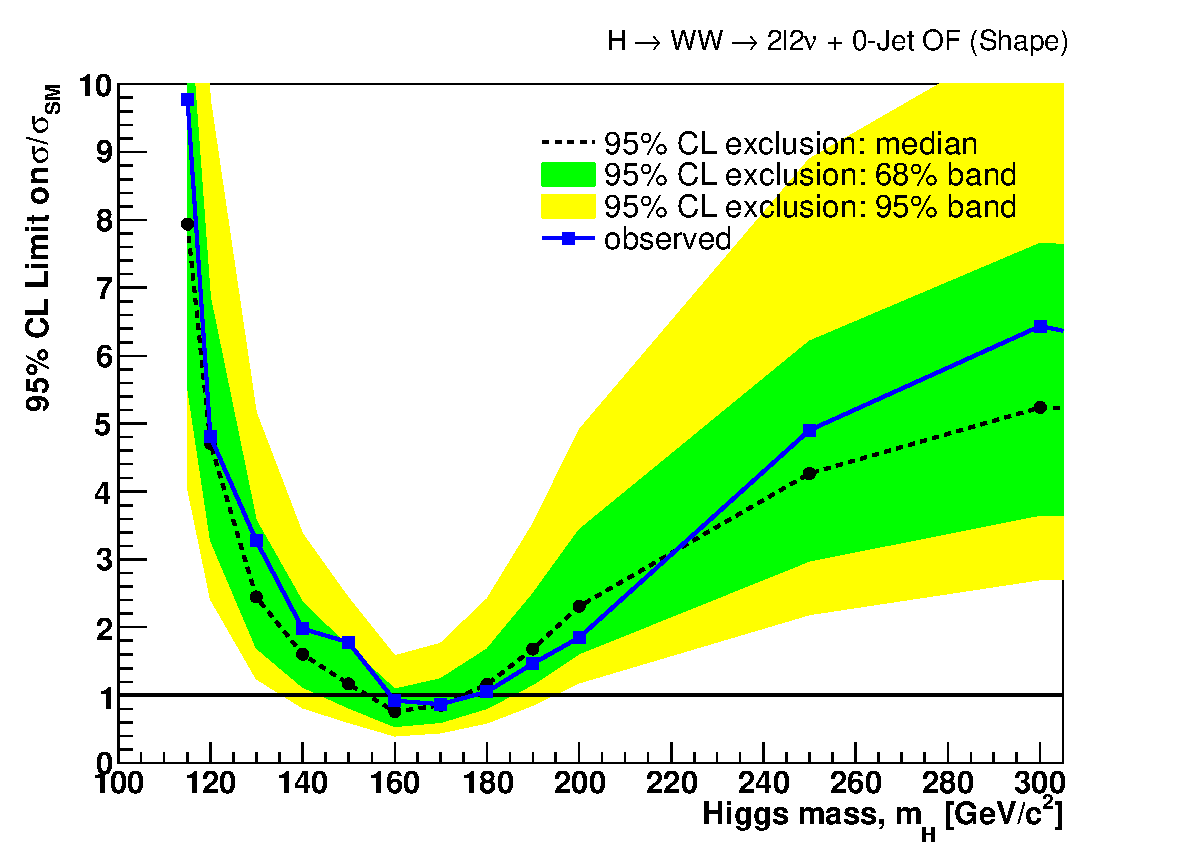
\includegraphics[width=0.48\textwidth]{lp_figures/limits_0j_of_shape_ana_v6_1500pb_LP_POSTEPS.pdf}}
\caption{Multivariate-based analysis upper limits at 95\% C.L. using LP, EPS and post-EPS datasets for 0-jet events.
\subref{subfig:lp_0j_sf_shape}: LP same-flavor; \subref{subfig:lp_0j_of_shape}: LP opposite-flavor;
\subref{subfig:eps_0j_sf_shape}: EPS same-flavor; \subref{subfig:eps_0j_of_shape}: EPS opposite-flavor;
\subref{subfig:post_0j_sf_shape}: post-EPS same-flavor; \subref{subfig:post_0j_of_shape}: post-EPS opposite-flavor;
}
\label{fig:limits_0j_shape}
\end{figure}

\subsubsection{One-Jet Cut-Based}
\begin{figure}[!htbp]
\centering
\subfigure[]{
\centering
\label{subfig:lp_1j_sf_cut}
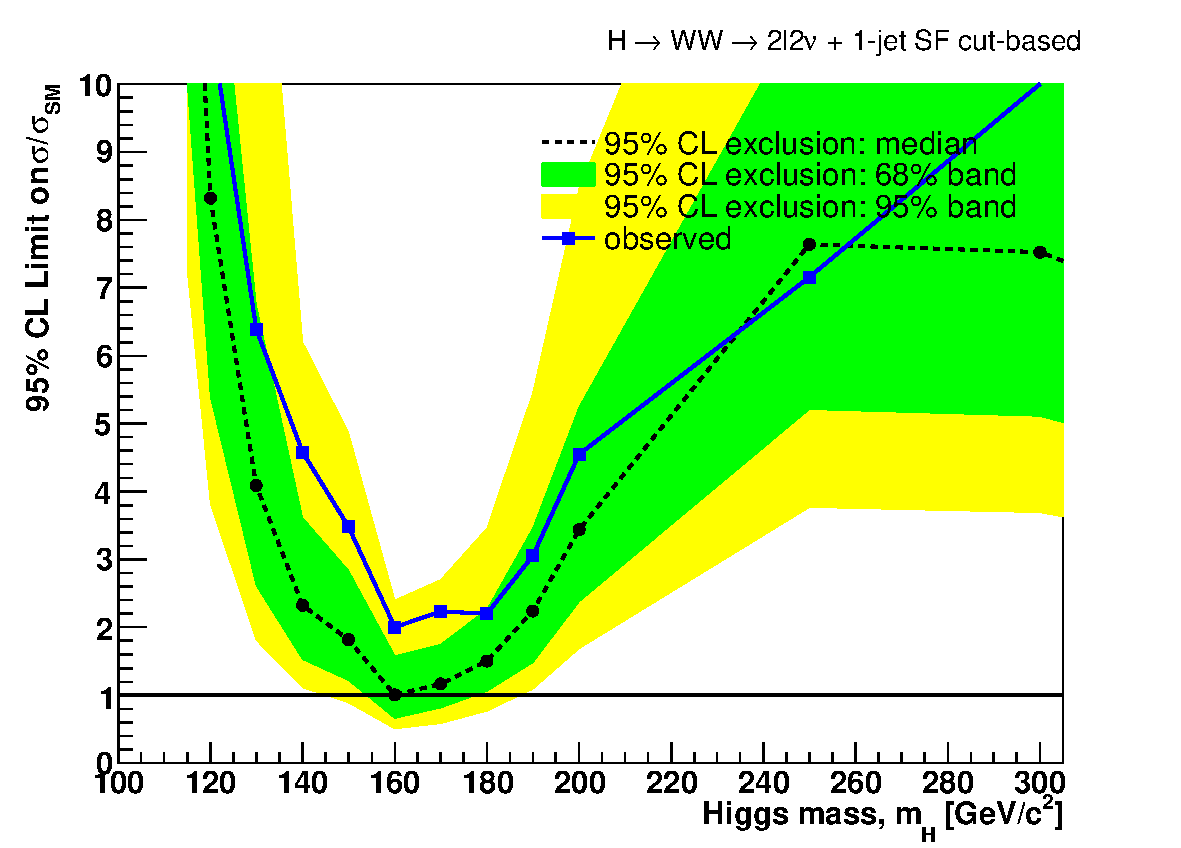
\includegraphics[width=0.48\textwidth]{lp_figures/limits_1j_sf_cut.pdf}}
\subfigure[]{
\centering
\label{subfig:lp_1j_of_cut}
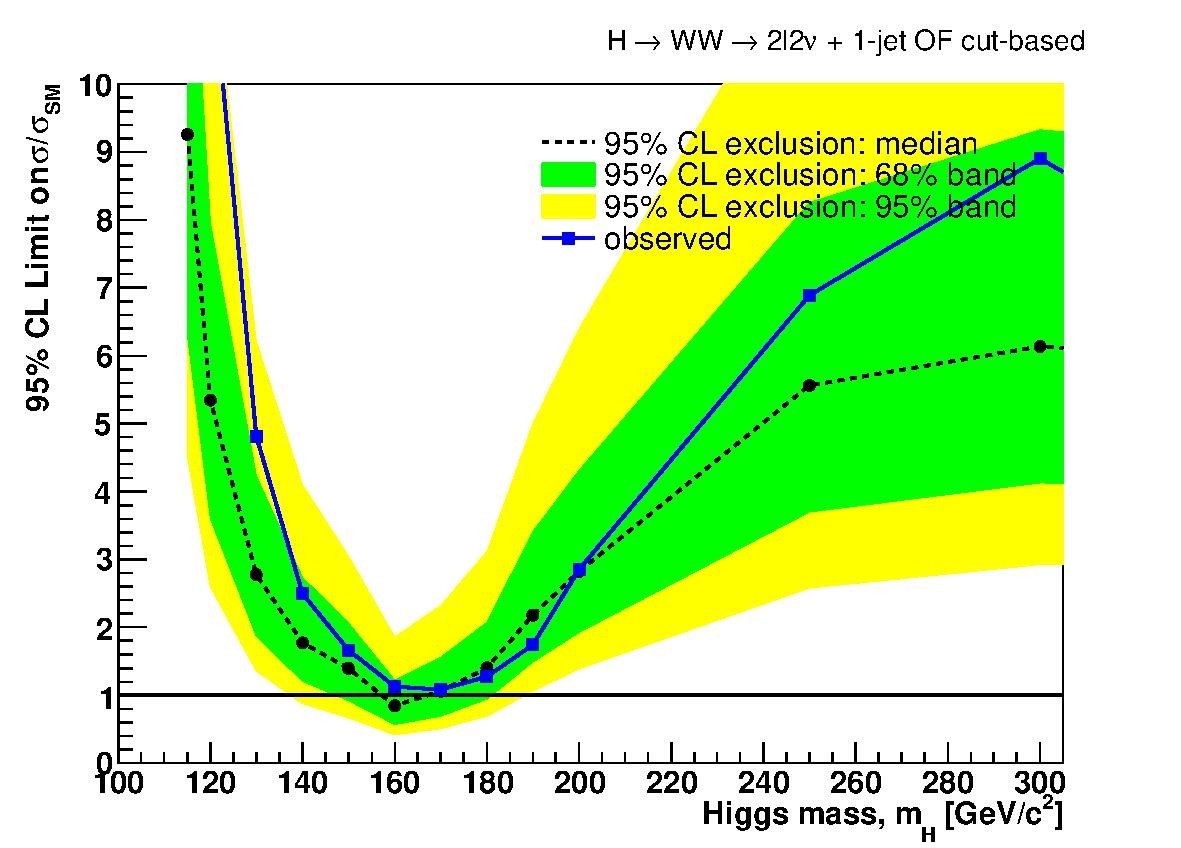
\includegraphics[width=0.48\textwidth]{lp_figures/limits_1j_of_cut.pdf}}
\subfigure[]{
\centering
\label{subfig:eps_1j_sf_cut}
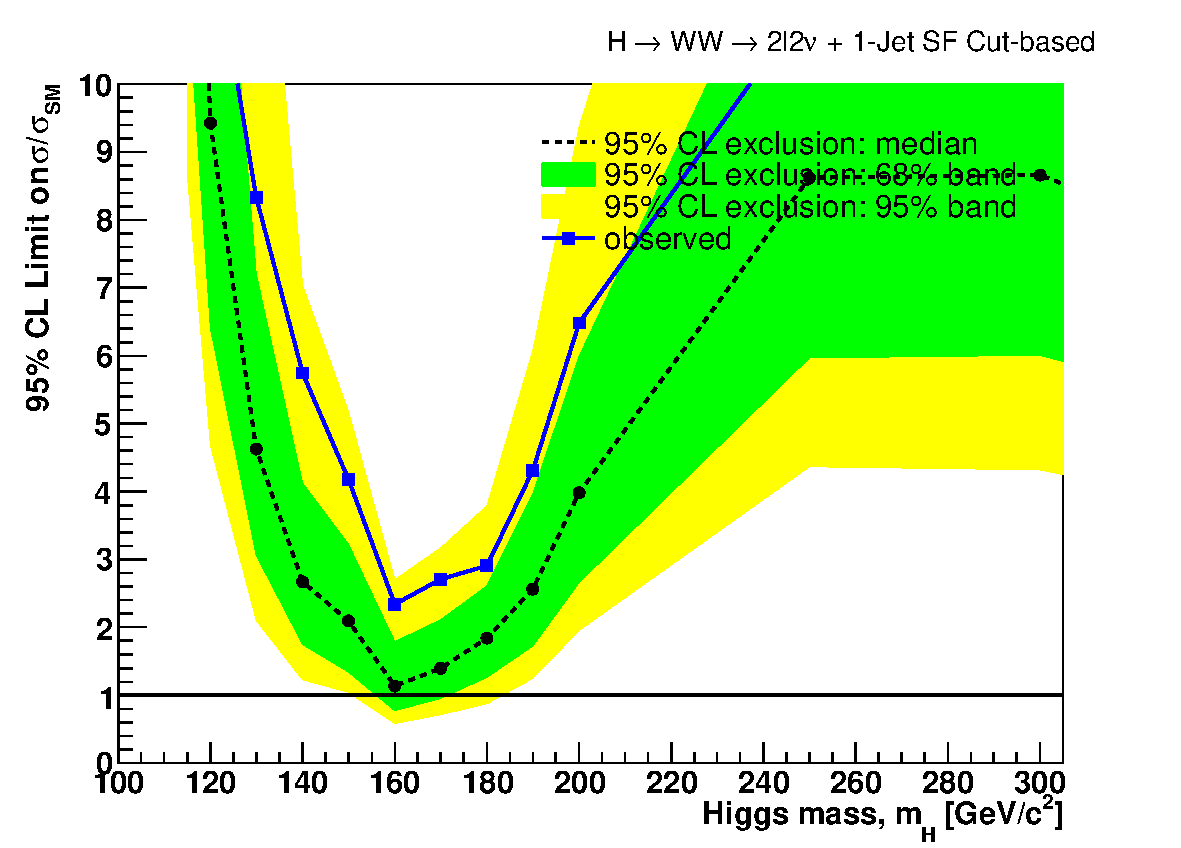
\includegraphics[width=0.48\textwidth]{lp_figures/limits_1j_sf_cut_ana_v6_1500pb_LP_EPS.pdf}}
\subfigure[]{
\centering
\label{subfig:eps_1j_of_cut}
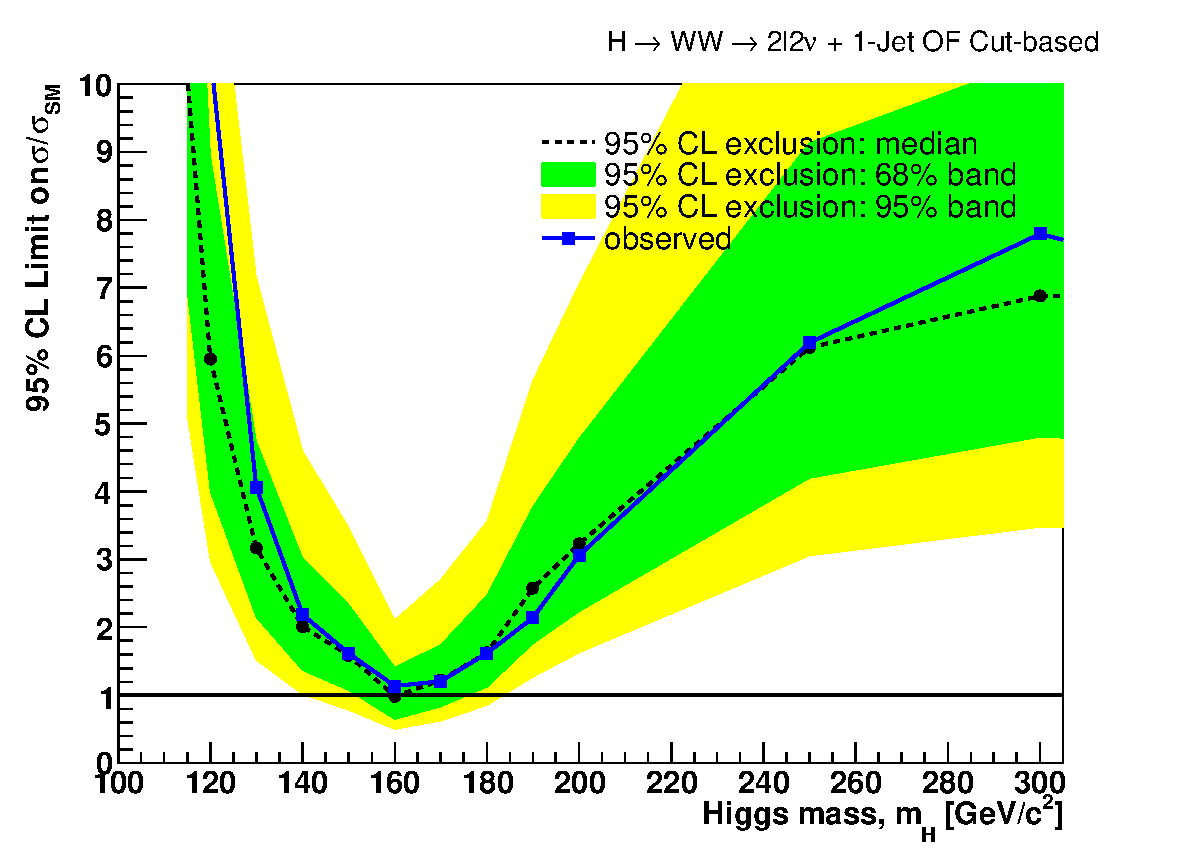
\includegraphics[width=0.48\textwidth]{lp_figures/limits_1j_of_cut_ana_v6_1500pb_LP_EPS.pdf}}
\subfigure[]{
\centering
\label{subfig:post_1j_sf_cut}
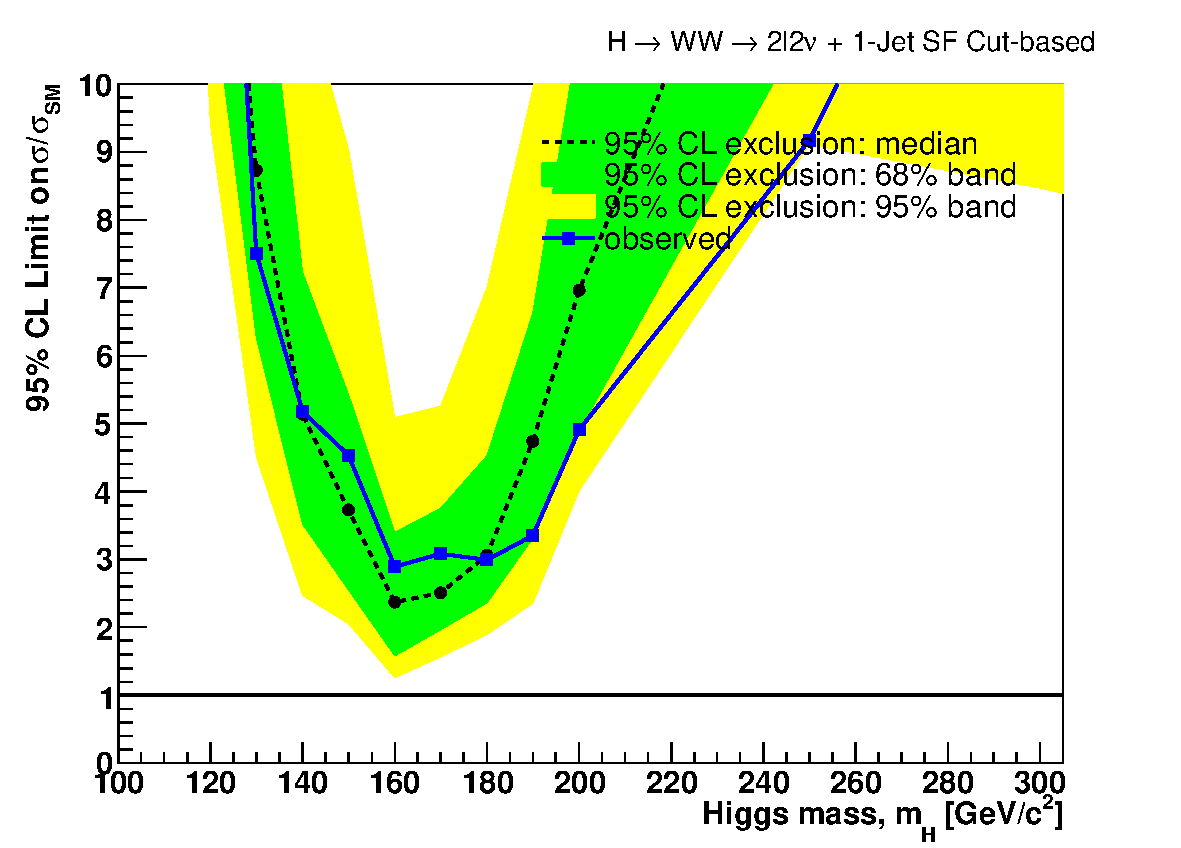
\includegraphics[width=0.48\textwidth]{lp_figures/limits_1j_sf_cut_ana_v6_1500pb_LP_POSTEPS.pdf}}
\subfigure[]{
\centering
\label{subfig:post_1j_of_cut}
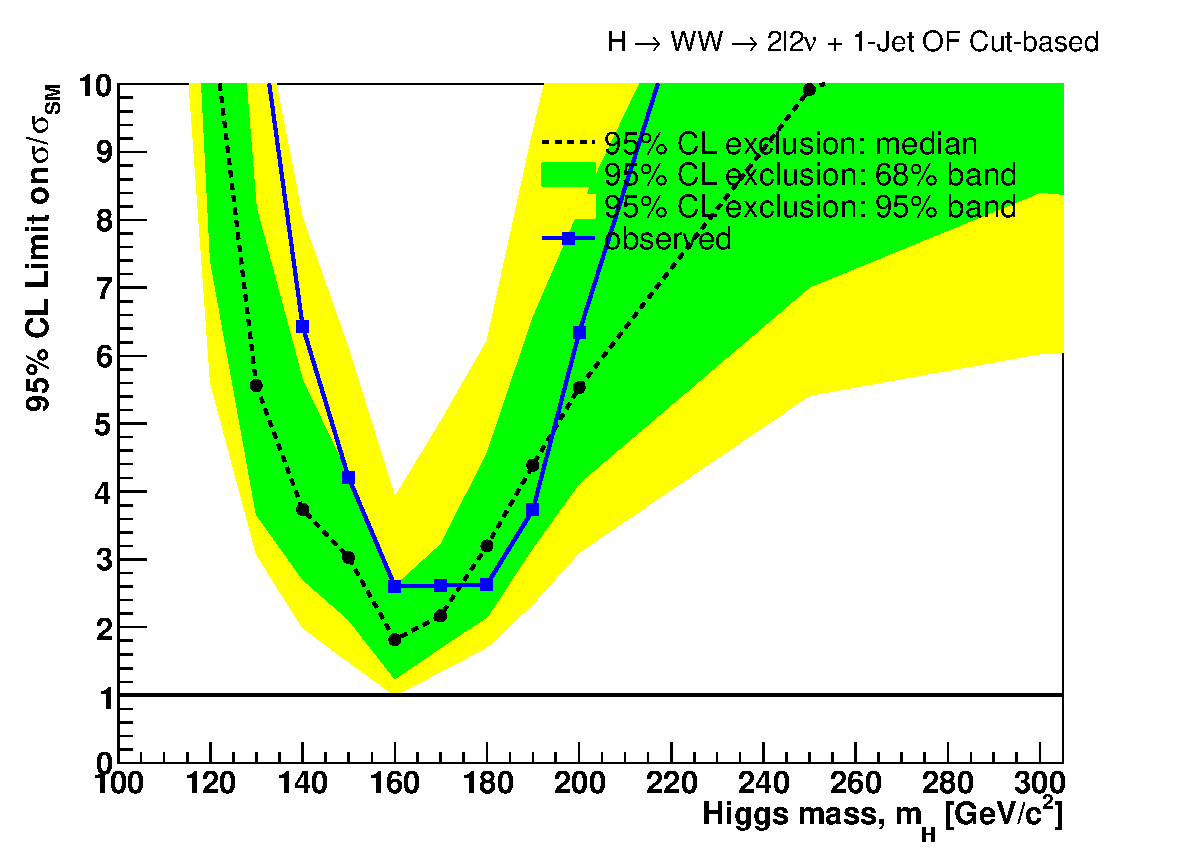
\includegraphics[width=0.48\textwidth]{lp_figures/limits_1j_of_cut_ana_v6_1500pb_LP_POSTEPS.pdf}}
\caption{Cut-based analysis upper limits at 95\% C.L. using LP, EPS and post-EPS datasets for 1-jet events.
\subref{subfig:lp_1j_sf_cut}: LP same-flavor; \subref{subfig:lp_1j_of_cut}: LP opposite-flavor;
\subref{subfig:eps_1j_sf_cut}: EPS same-flavor; \subref{subfig:eps_1j_of_cut}: EPS opposite-flavor;
\subref{subfig:post_1j_sf_cut}: post-EPS same-flavor; \subref{subfig:post_1j_of_cut}: post-EPS opposite-flavor;
}
\label{fig:limits_1j_cut}
\end{figure}

\subsubsection{One-Jet MVA-Based}
\begin{figure}[!htbp]
\centering
\subfigure[]{
\centering
\label{subfig:lp_1j_sf_shape}
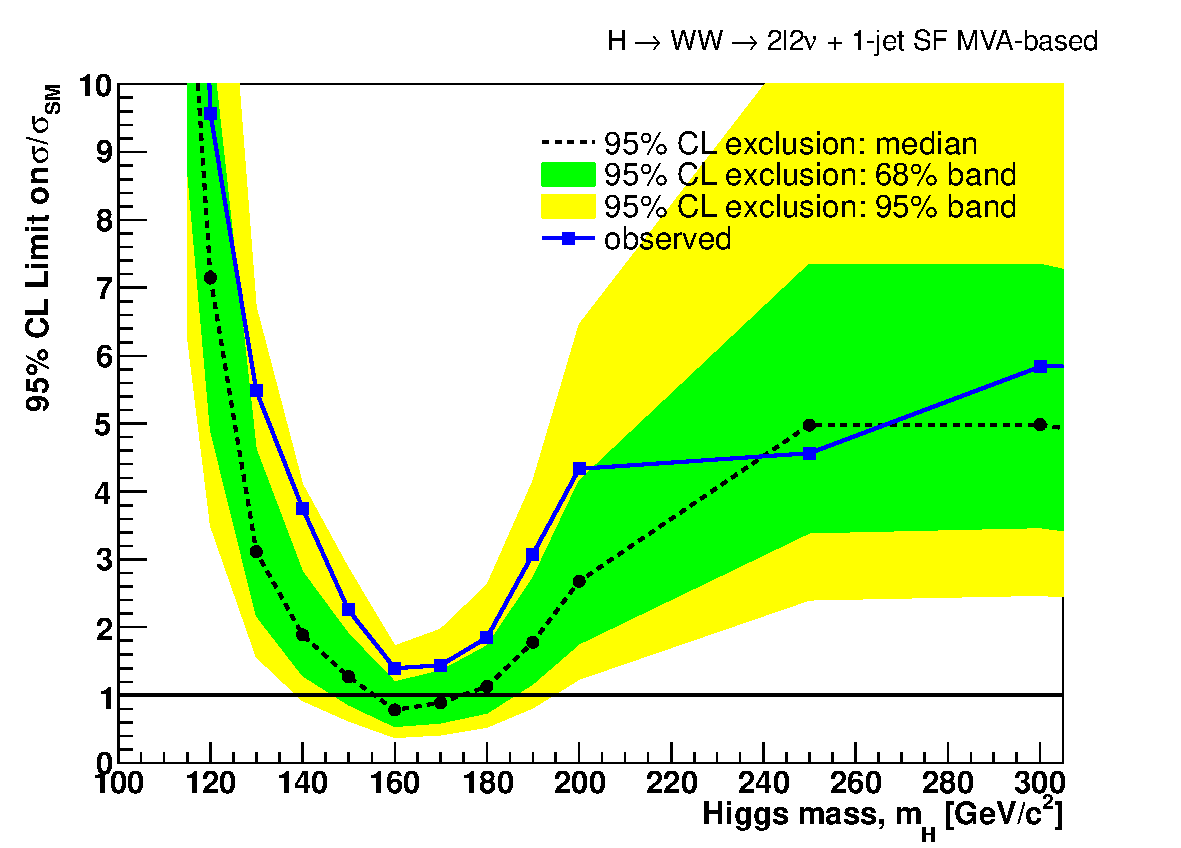
\includegraphics[width=0.48\textwidth]{lp_figures/limits_1j_sf_shape.pdf}}
\subfigure[]{
\centering
\label{subfig:lp_1j_of_shape}
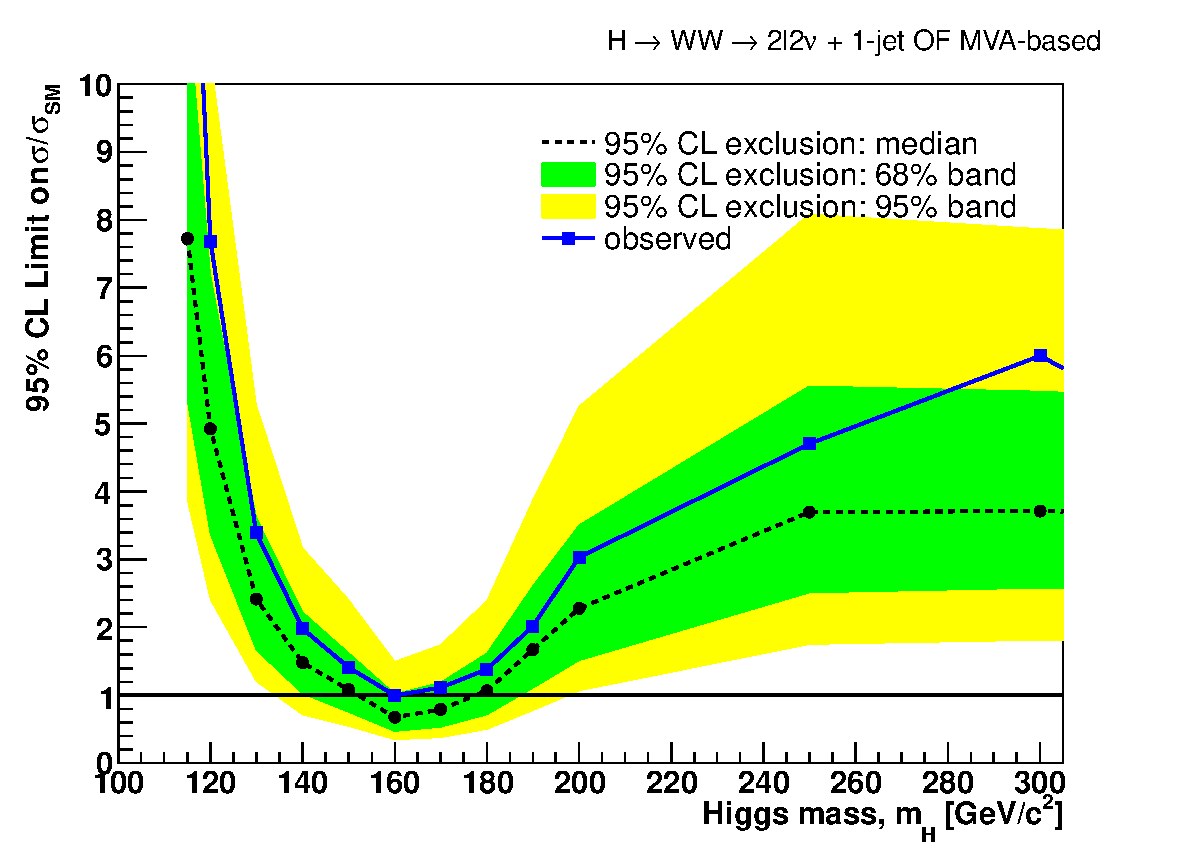
\includegraphics[width=0.48\textwidth]{lp_figures/limits_1j_of_shape.pdf}}
\subfigure[]{
\centering
\label{subfig:eps_1j_sf_shape}
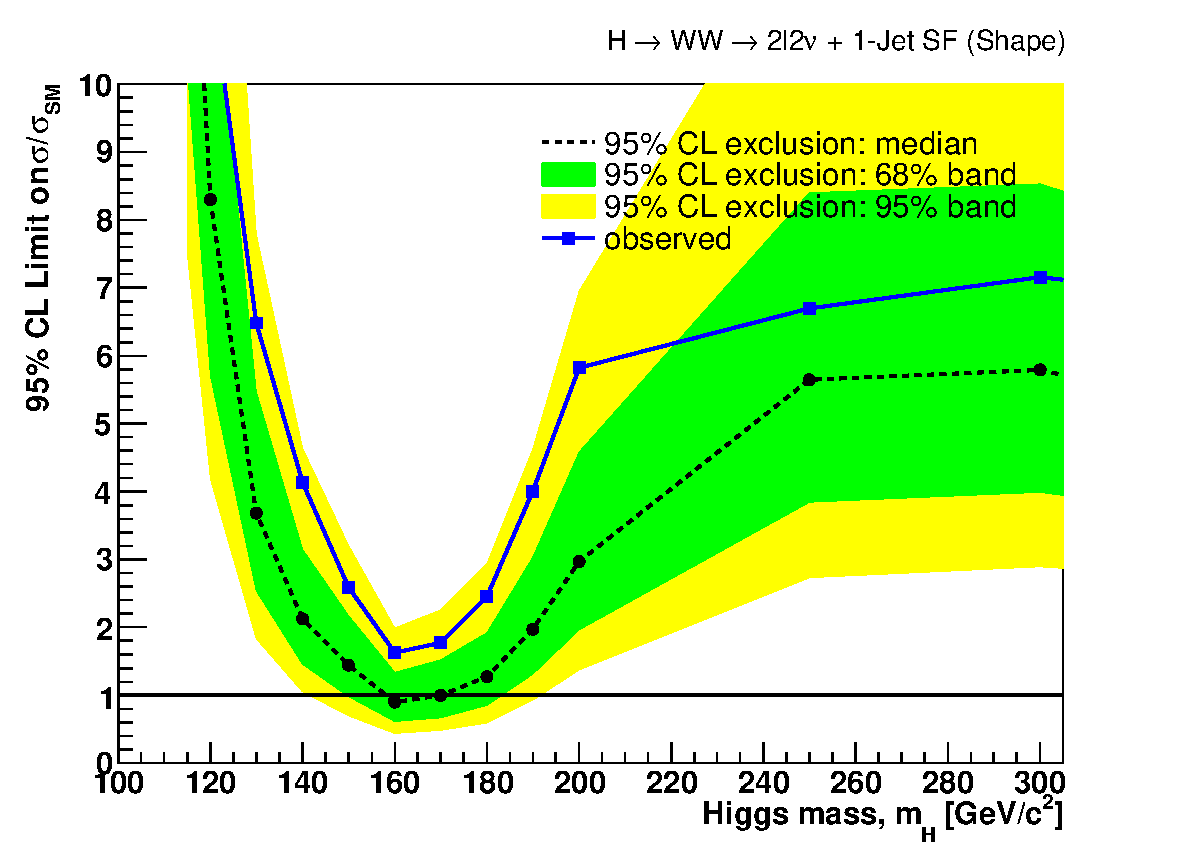
\includegraphics[width=0.48\textwidth]{lp_figures/limits_1j_sf_shape_ana_v6_1500pb_LP_EPS.pdf}}
\subfigure[]{
\centering
\label{subfig:eps_1j_of_shape}
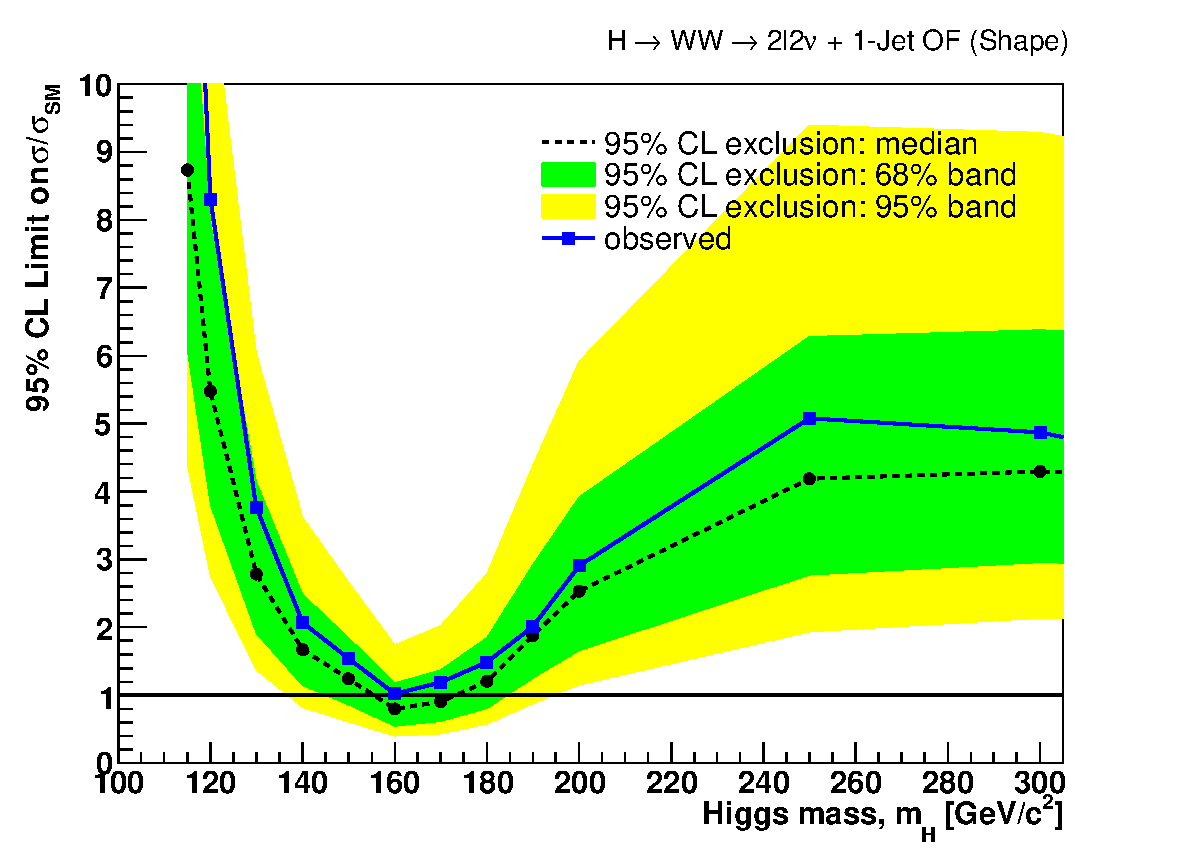
\includegraphics[width=0.48\textwidth]{lp_figures/limits_1j_of_shape_ana_v6_1500pb_LP_EPS.pdf}}
\subfigure[]{
\centering
\label{subfig:post_1j_sf_shape}
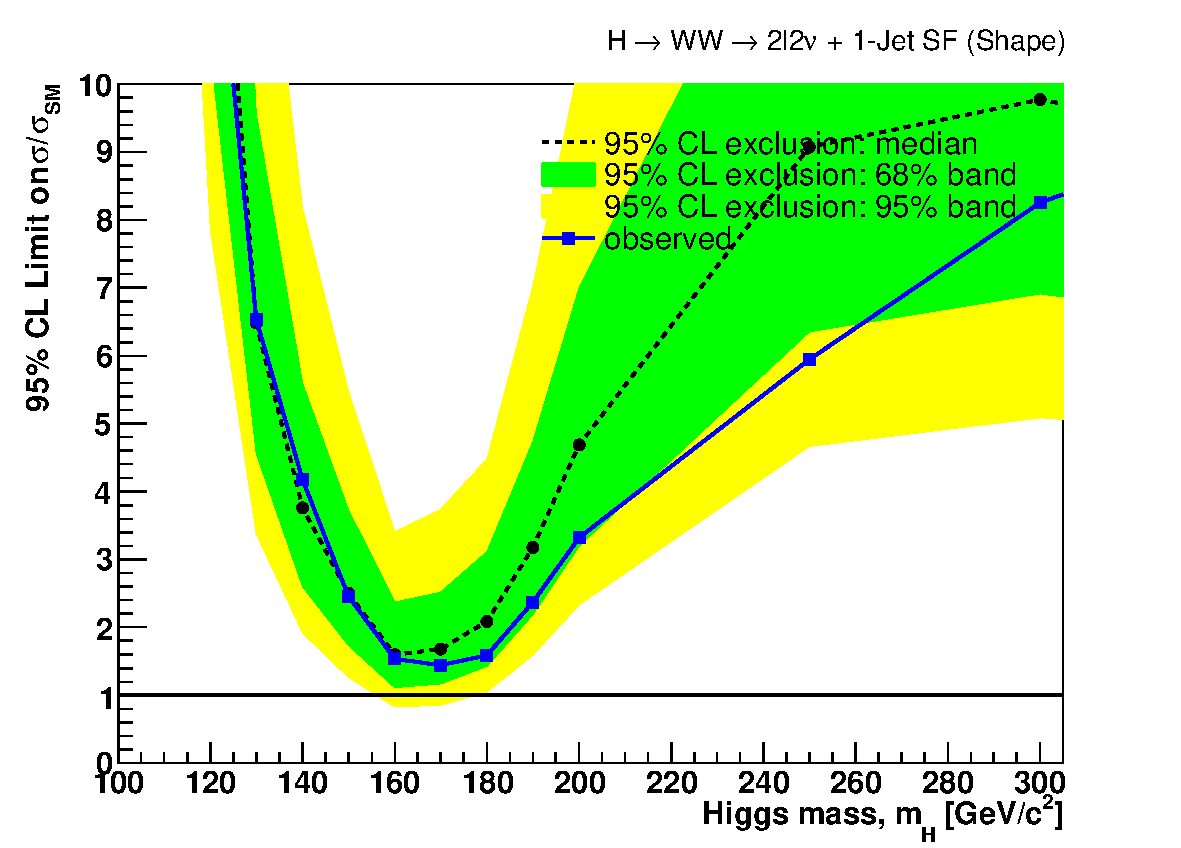
\includegraphics[width=0.48\textwidth]{lp_figures/limits_1j_sf_shape_ana_v6_1500pb_LP_POSTEPS.pdf}}
\subfigure[]{
\centering
\label{subfig:post_1j_of_shape}
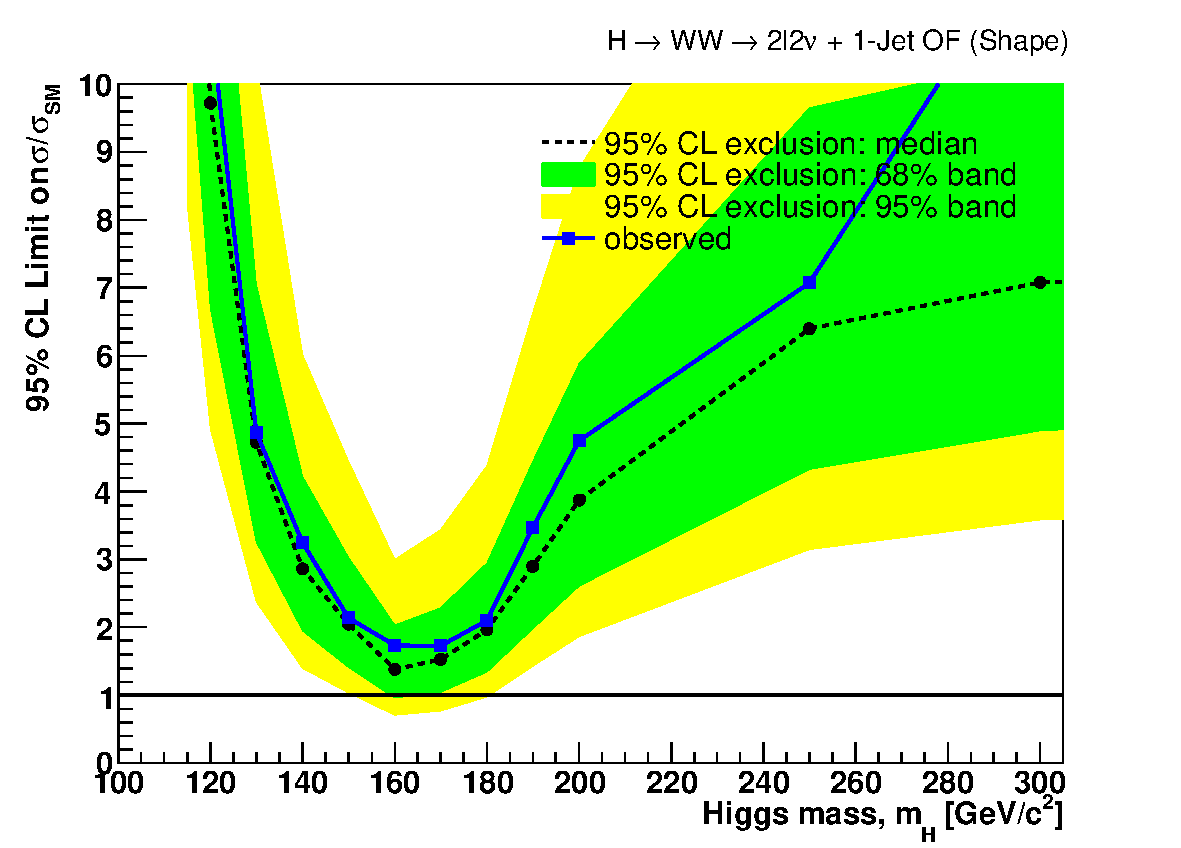
\includegraphics[width=0.48\textwidth]{lp_figures/limits_1j_of_shape_ana_v6_1500pb_LP_POSTEPS.pdf}}
\caption{Multivariate-based analysis upper limits at 95\% C.L. using LP, EPS and post-EPS datasets for 1-jet events.
\subref{subfig:lp_1j_sf_shape}: LP same-flavor; \subref{subfig:lp_1j_of_shape}: LP opposite-flavor;
\subref{subfig:eps_1j_sf_shape}: EPS same-flavor; \subref{subfig:eps_1j_of_shape}: EPS opposite-flavor;
\subref{subfig:post_1j_sf_shape}: post-EPS same-flavor; \subref{subfig:post_1j_of_shape}: post-EPS opposite-flavor;
}
\label{fig:limits_1j_shape}
\end{figure}


%%%%%%%%%%%%%%%%%%%%%%%%%%%%%%
\subsubsection{Cut-Based with Additional Transverse Mass Requirement}
\begin{figure}[!htbp]
\centering
\subfigure[]{
\centering
\label{subfig:0j_sf}
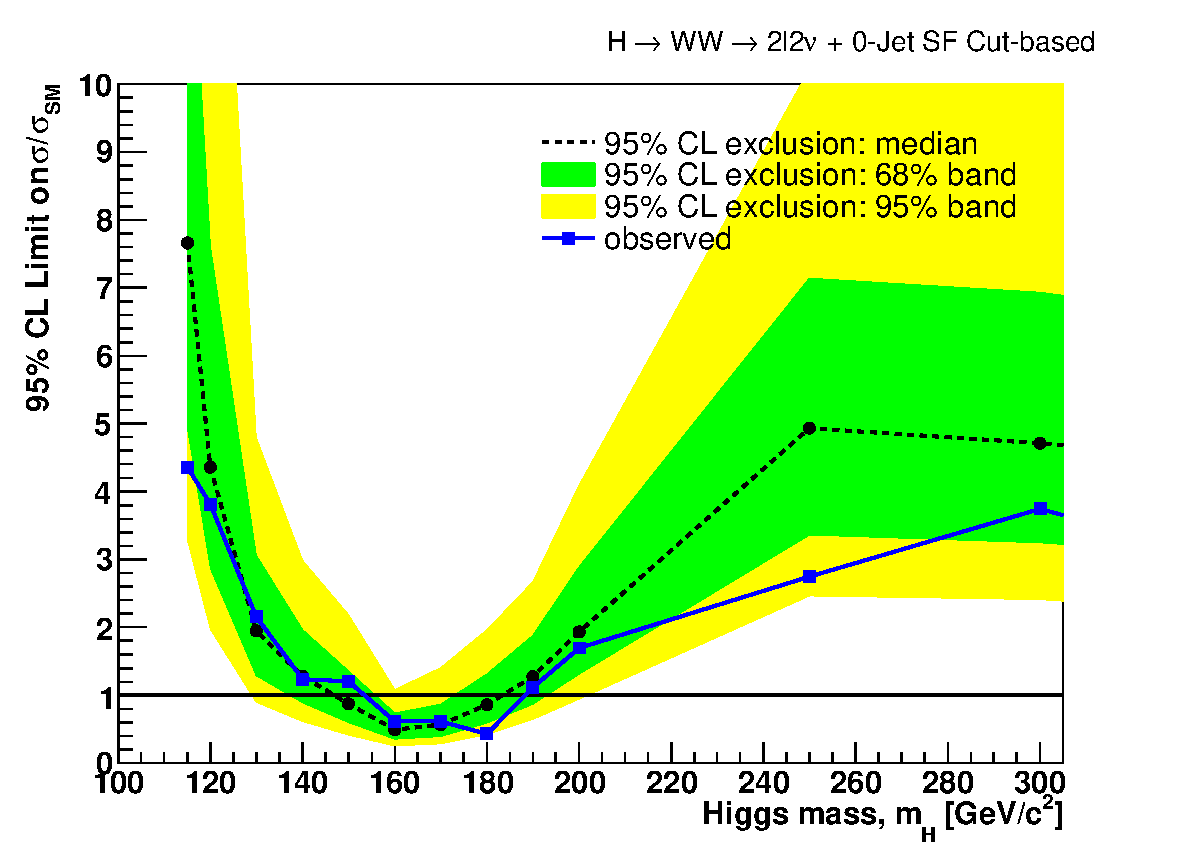
\includegraphics[width=0.48\textwidth]{lp_figures/limits_0j_sf_cut_ana_v6_1500pb_LP_MTCUT80.pdf}}
\subfigure[]{
\centering
\label{subfig:0j_of}
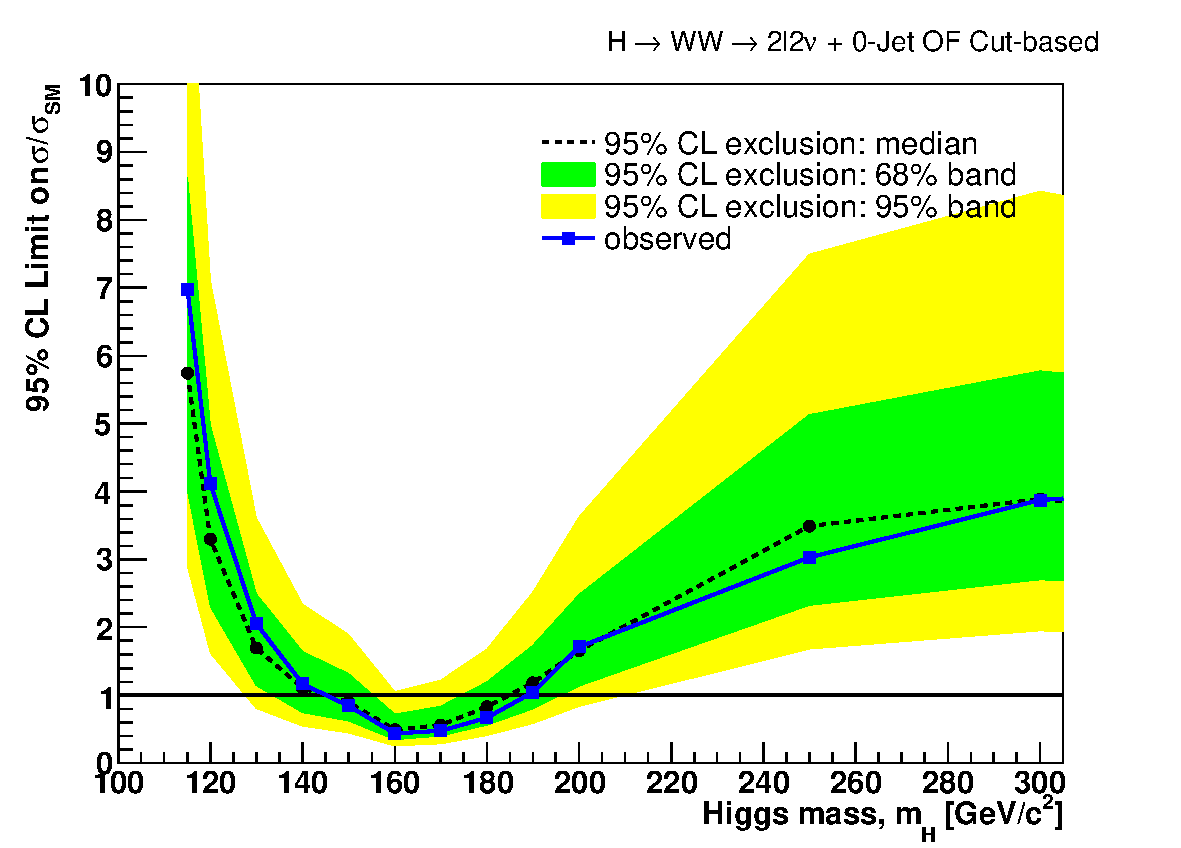
\includegraphics[width=0.48\textwidth]{lp_figures/limits_0j_of_cut_ana_v6_1500pb_LP_MTCUT80.pdf}}
\subfigure[]{
\centering
\label{subfig:1j_sf}
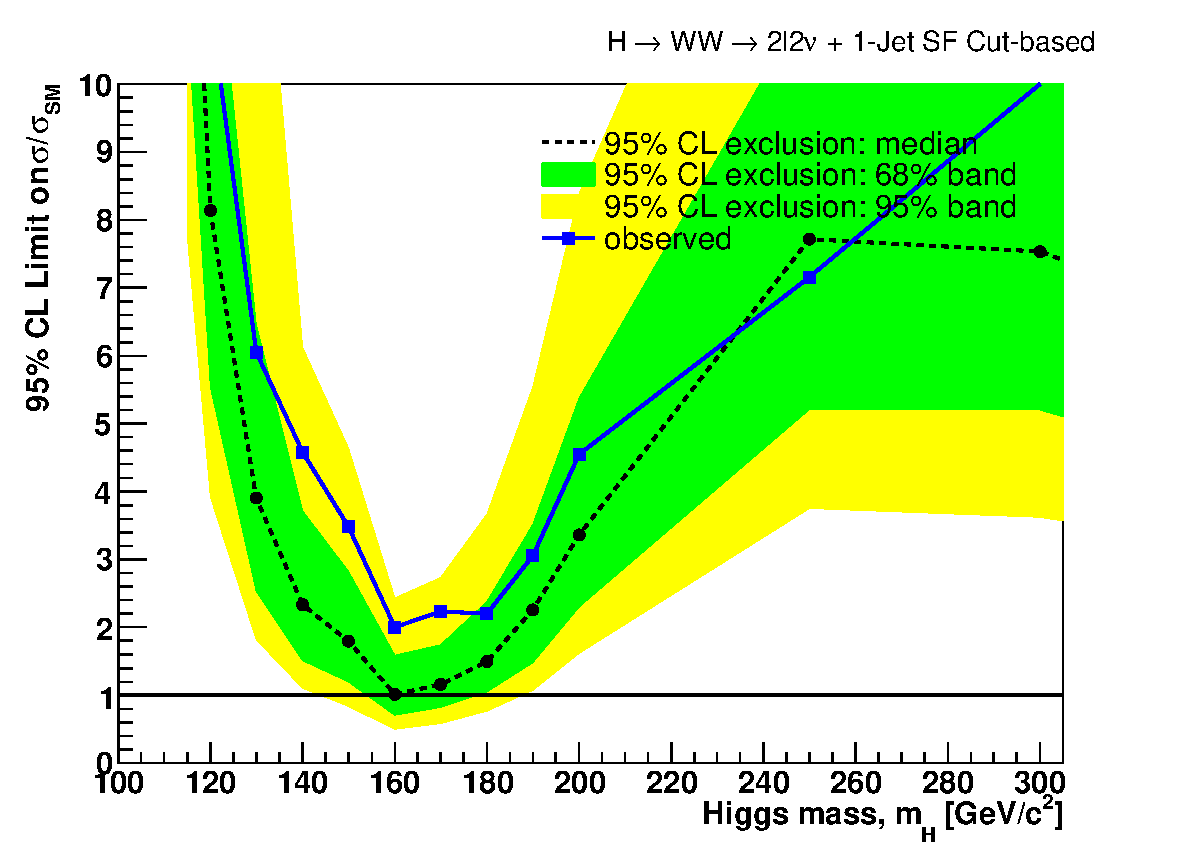
\includegraphics[width=0.48\textwidth]{lp_figures/limits_1j_sf_cut_ana_v6_1500pb_LP_MTCUT80.pdf}}
\subfigure[]{
\centering
\label{subfig:1j_of}
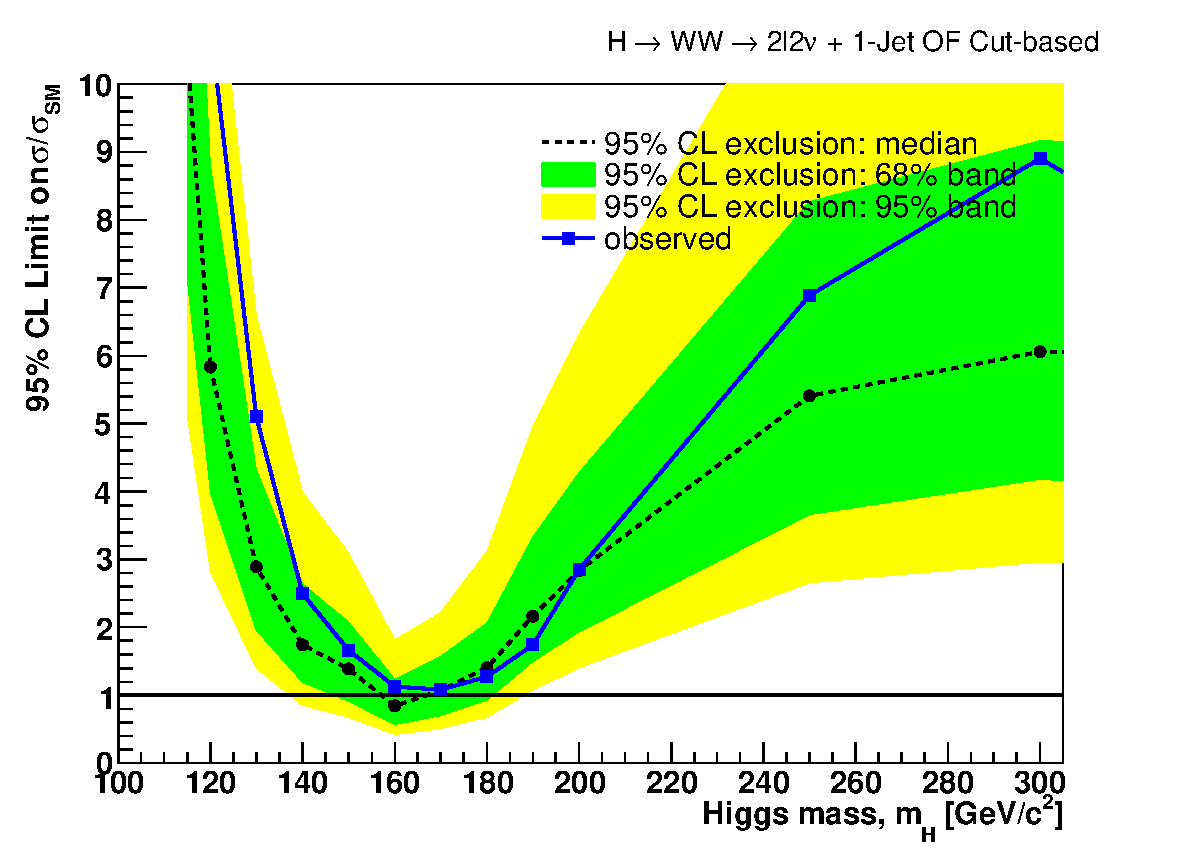
\includegraphics[width=0.48\textwidth]{lp_figures/limits_1j_of_cut_ana_v6_1500pb_LP_MTCUT80.pdf}}
\subfigure[]{
\centering
\label{subfig:2j}
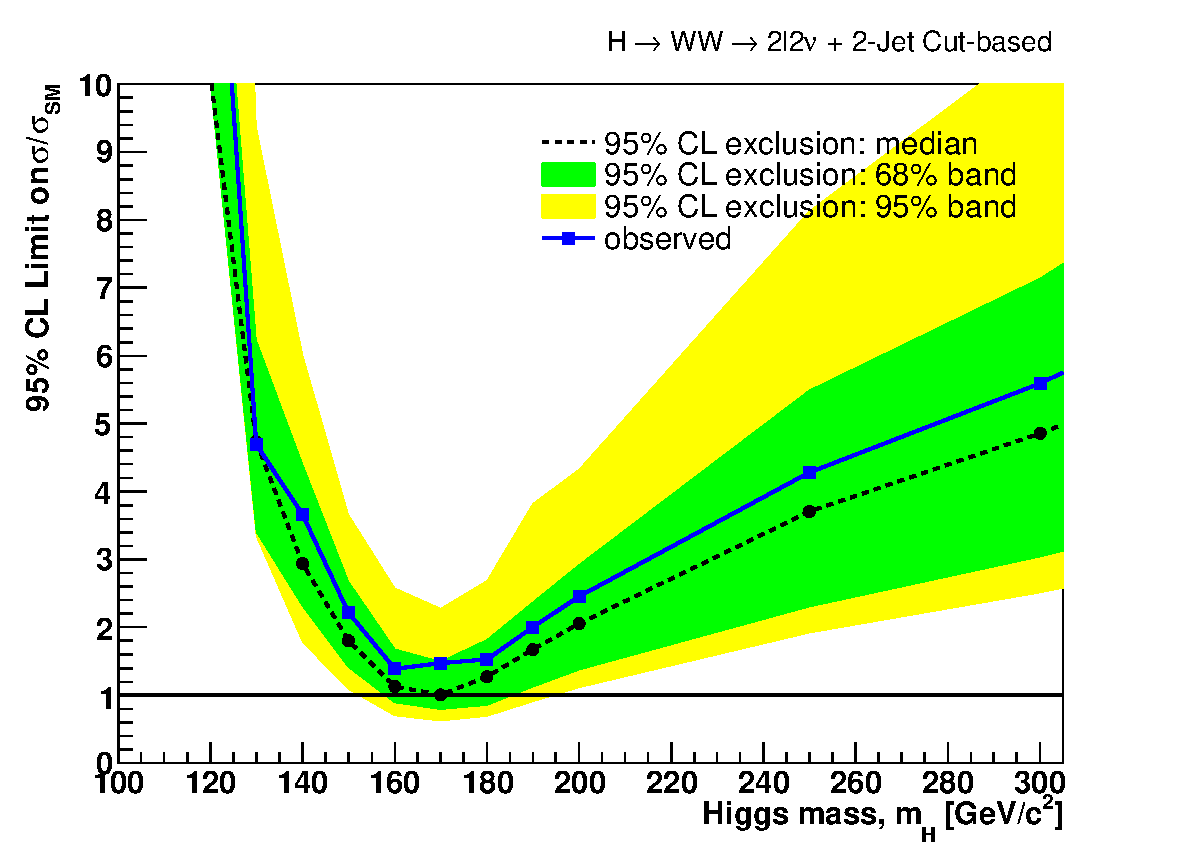
\includegraphics[width=0.48\textwidth]{lp_figures/limits_2j_cut_ana_v6_1500pb_LP_MTCUT80.pdf}}
\subfigure[]{
\centering
\label{subfig:njcomb}
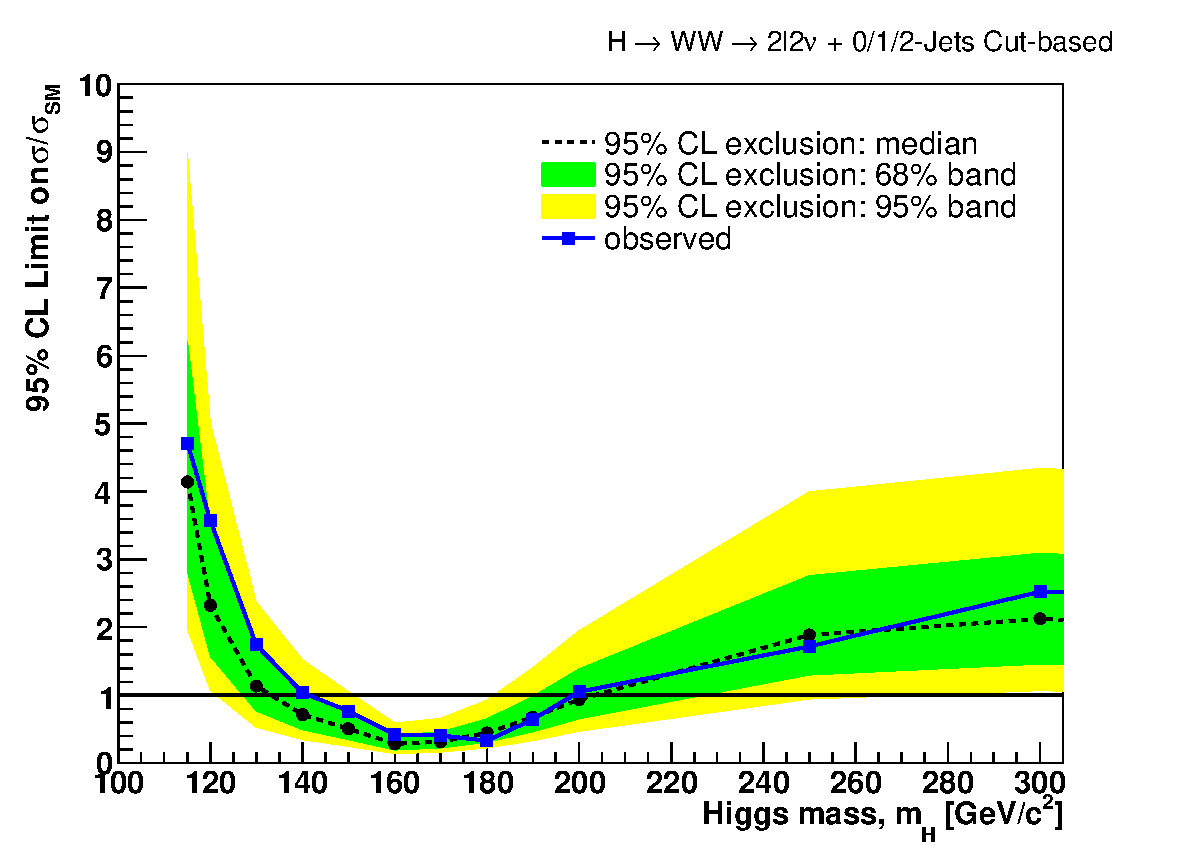
\includegraphics[width=0.48\textwidth]{lp_figures/limits_nj_cut_ana_v6_1500pb_LP_MTCUT80.pdf}}
\caption{Cut-based analysis upper limits at 95\% C.L. using data corresponding to 1.5~$\ifb$ applying the additional $m_T$ cut.
The limits are shown in 4 final states separately. \subref{subfig:0j_sf}: SF in 0 Jet bin;
\subref{subfig:0j_of}: OF in 0 Jet bin; \subref{subfig:1j_sf}: SF in 1 Jet bin;
\subref{subfig:1j_of}: OF in 1 Jet bin; \subref{subfig:2j}: 2 Jet bin; \subref{subfig:njcomb}: 0/1/2 Jets combined; }
\label{fig:limits_lp_mtcut80_cut}
\end{figure}
%%%%%%%%%%%%%%%%%%%%%%%%%%%%%%

\subsubsection{MVA-Based with Additional Transverse Mass Requirement}
\begin{figure}[!htbp]
\centering
\subfigure[]{
\centering
\label{subfig:0j_sf}
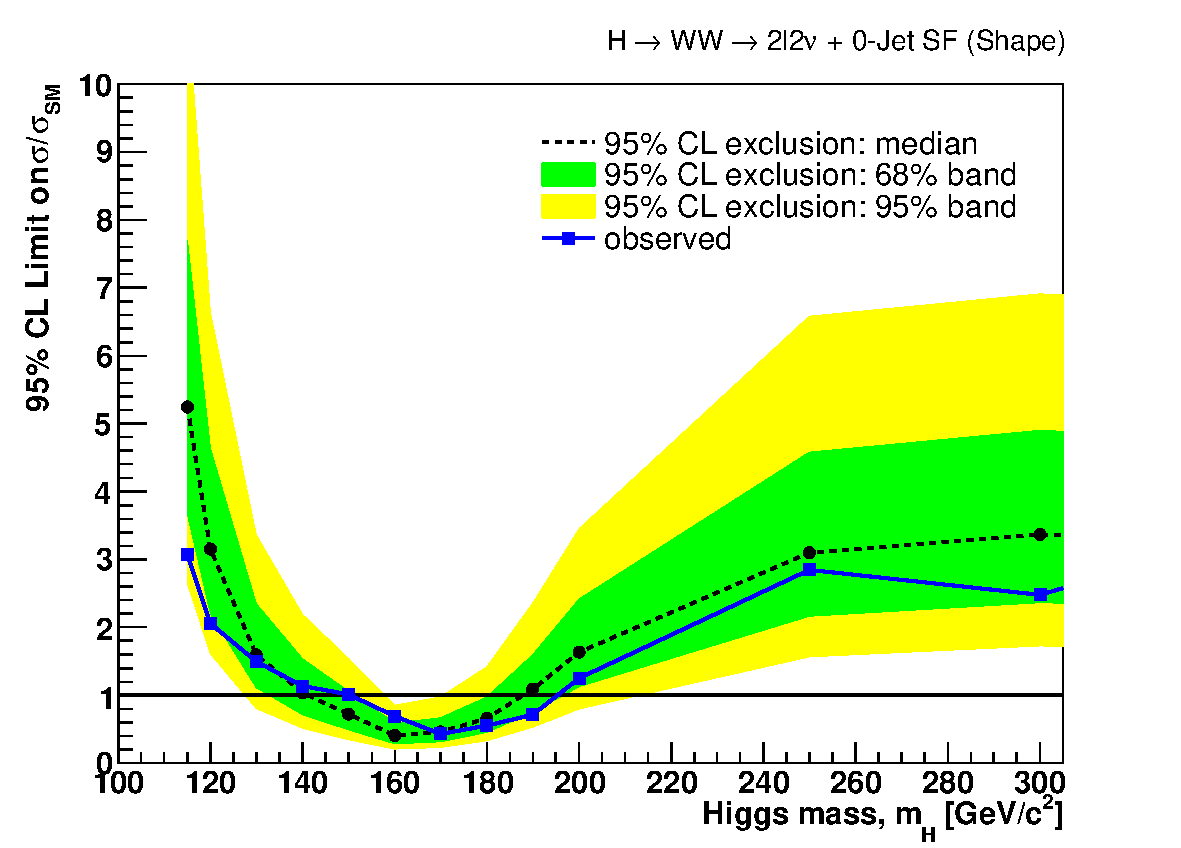
\includegraphics[width=0.48\textwidth]{lp_figures/limits_0j_sf_shape_ana_v6_1500pb_LP_MTCUT80.pdf}
}
\subfigure[]{
\centering
\label{subfig:0j_of}
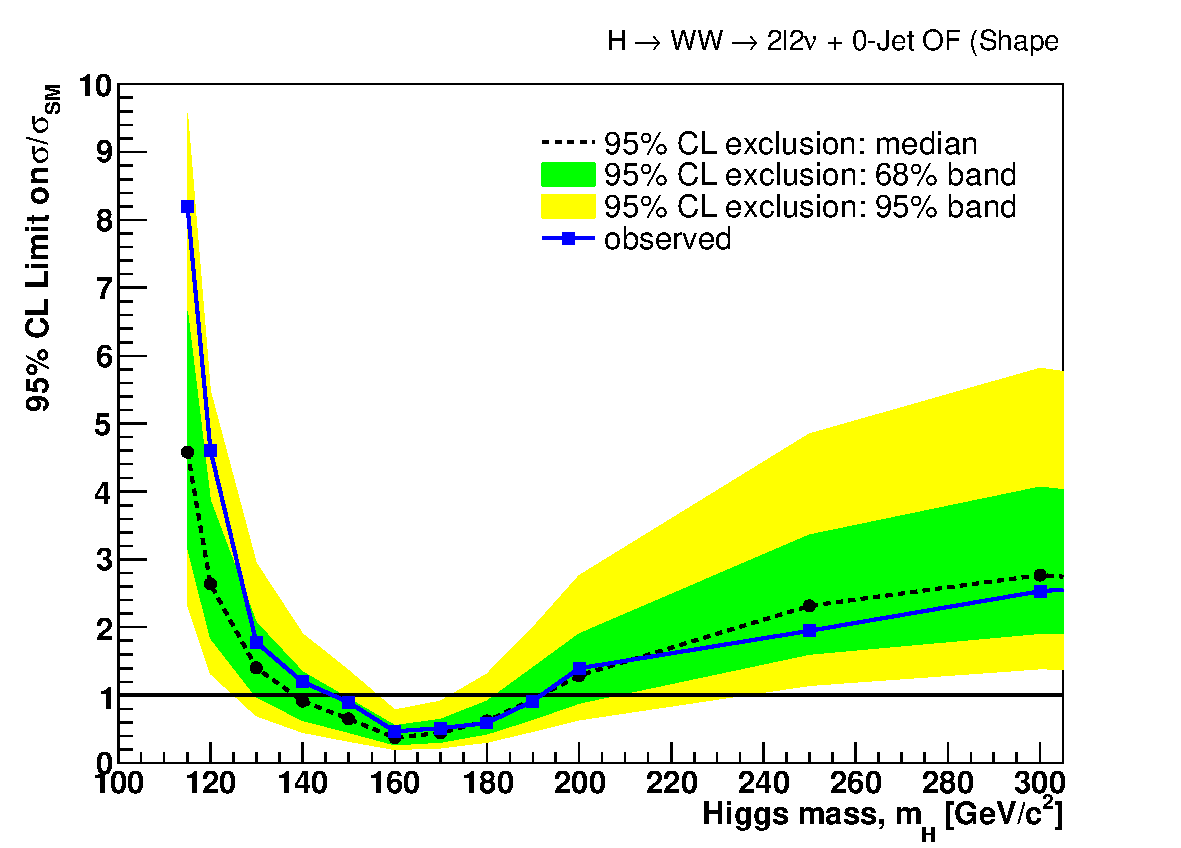
\includegraphics[width=0.48\textwidth]{lp_figures/limits_0j_of_shape_ana_v6_1500pb_LP_MTCUT80.pdf}
}
\subfigure[]{
\centering
\label{subfig:1j_sf}
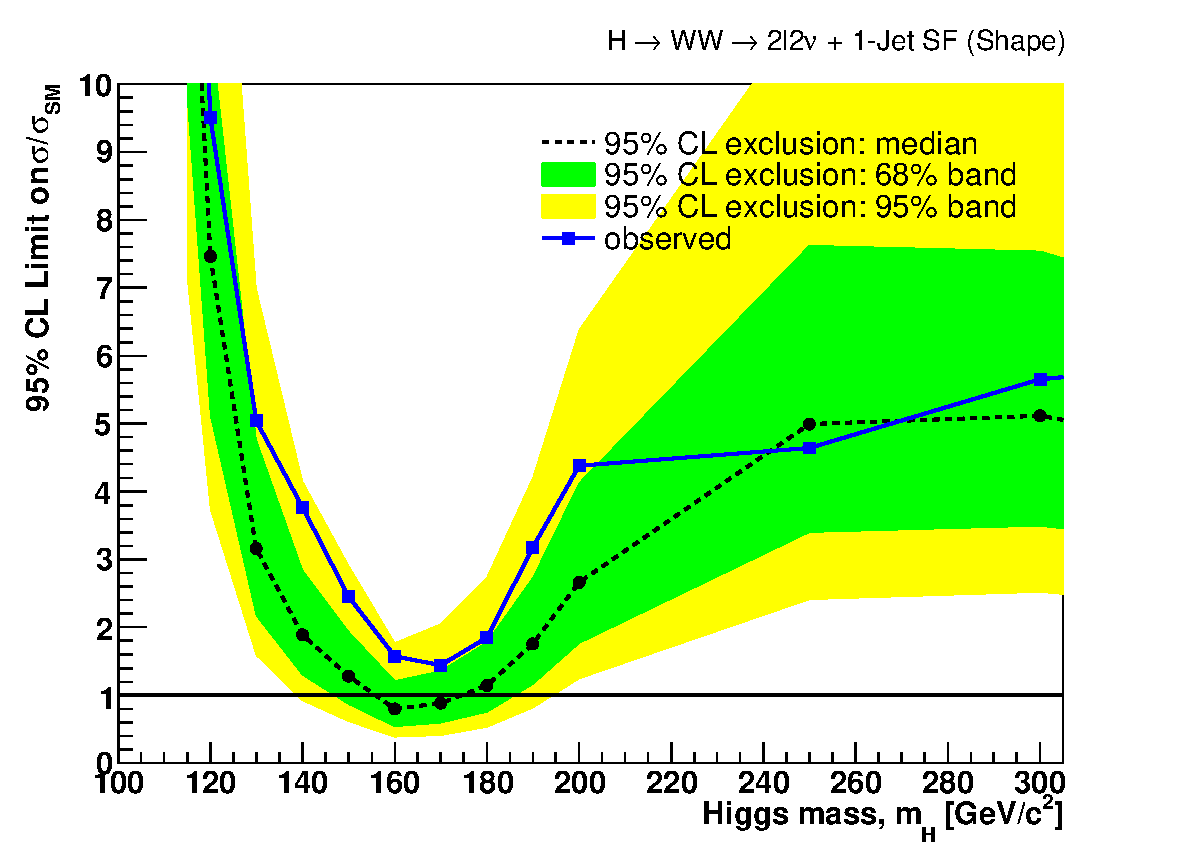
\includegraphics[width=0.48\textwidth]{lp_figures/limits_1j_sf_shape_ana_v6_1500pb_LP_MTCUT80.pdf}
}
\subfigure[]{
\centering
\label{subfig:1j_of}
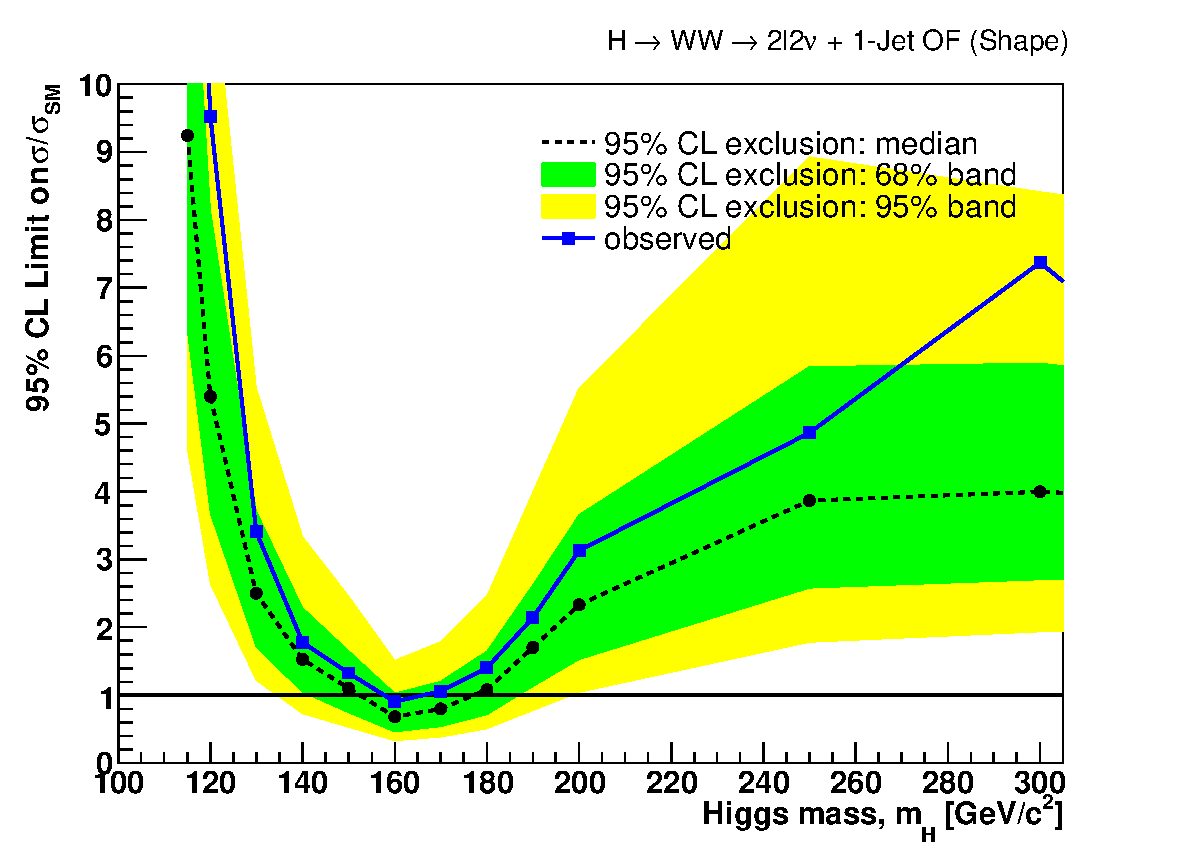
\includegraphics[width=0.48\textwidth]{lp_figures/limits_1j_of_shape_ana_v6_1500pb_LP_MTCUT80.pdf}
}
\subfigure[]{
\centering
\label{subfig:nj}
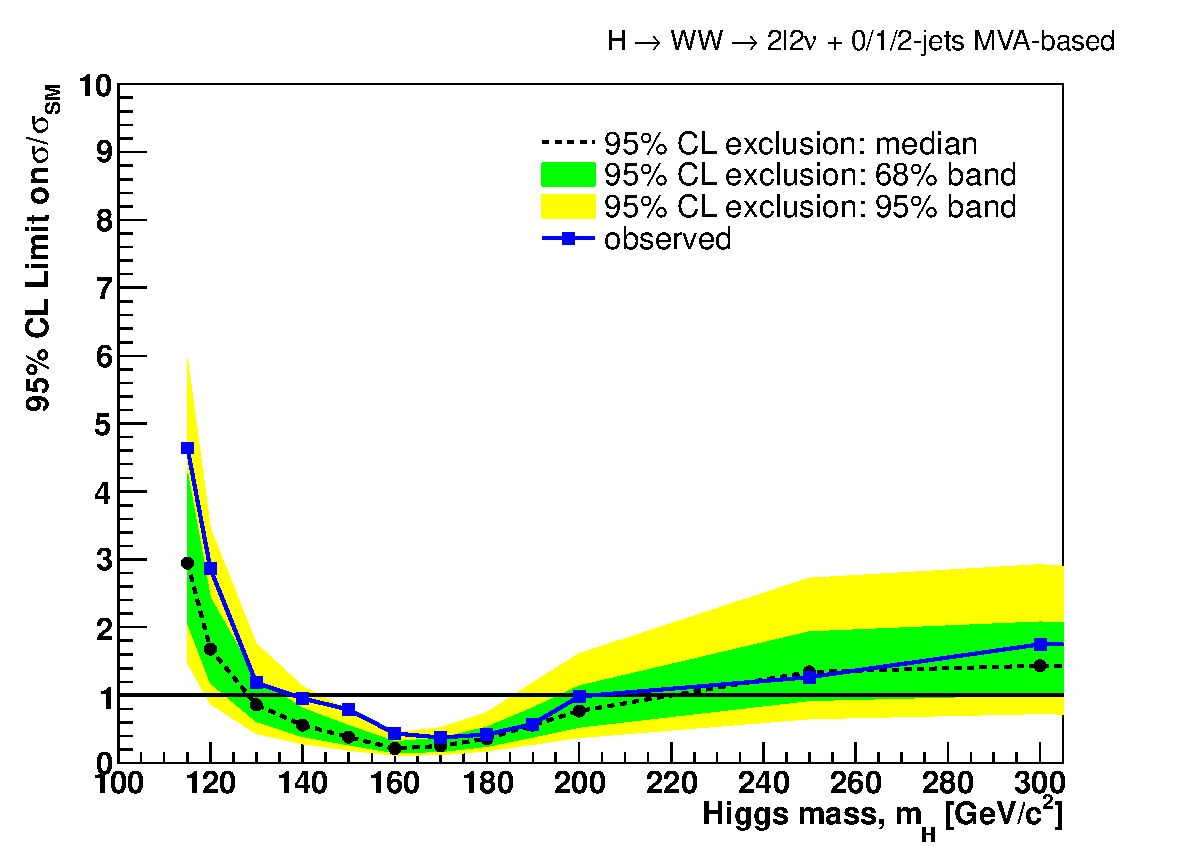
\includegraphics[width=0.48\textwidth]{lp_figures/limits_nj_shape_ana_v6_1500pb_LP_MTCUT80.pdf}
}
\caption{Multivariate based analysis upper limits at 95\% C.L. using data corresponding to 1.5~$\ifb$,
applying the additional $m_T$ cut.
The limits are shown in 4 final states separately. \subref{subfig:0j_sf}: SF in 0 Jet bin;
\subref{subfig:0j_of}: OF in 0 Jet bin; \subref{subfig:1j_sf}: SF in 1 Jet bin;
\subref{subfig:1j_of}: OF in 1 Jet bin; \subref{subfig:nj}: 0/1/2 Jets combined;
}
\label{fig:limits_lp_mtcut80_shape}
\end{figure}

%%%%%%%%%%%%%%%%%%%%%%%%%%%%%%

\subsection{Tabulated Limits}
\subsubsection{}



